%\documentclass{beamer}
\documentclass[xcolor={dvipsnames,svgnames,table}]{beamer}

\usepackage[brazil]{babel}
\usepackage[utf8]{inputenc}

\usepackage{xcolor}
\usepackage{enumitem,xcolor}
\usepackage{subfig}
\usepackage{comment}
\usepackage{enumitem}
\usepackage{amsmath}
\usepackage{amsfonts}
\usepackage{amssymb}
\usepackage{graphicx}
\usepackage{ragged2e}
%\usepackage{floatrow}
\usepackage{etoolbox}
\usepackage{graphics}
\usepackage{booktabs}
\usepackage{multirow}
%\usepackage[small]{caption} 

\usetheme{Madrid}
\usecolortheme{seahorse}

\usefonttheme{professionalfonts}

%\newcommand\Fontvi{\fontsize{6}{7.2}\selectfont}

%\usepackage{newtxtext,newtxmath}

%cor
\setbeamercolor{structure}{bg=White,fg=Green!50!Black}
\setbeamercolor{palette primary}{fg=White,bg=Green!75!Black}
\setbeamercolor{palette secondary}{fg=White,bg=Green!60!Black}
\setbeamercolor{palette tertiary}{fg=White,bg=Green!75!Black}
\setbeamercolor{alerted text}{fg=DarkRed}

\setbeamercolor{title}{fg=White,bg=Green!70!Black}
\setbeamercolor{frametitle}{fg=White,bg=Green!50!Black}

\setbeamercolor{block title}{fg=White,bg=Green!50!Black}
\setbeamercolor{block body}{fg=Black,bg=Green!25!White}

\setbeamercolor{block title example}{fg=White,bg=Green!50!Black}
\setbeamercolor{block body example}{fg=Black,bg=Green!25!White}

\setbeamerfont{title}{size=\normalsize,series=\bfseries}
\setbeamerfont{frametitle}{size=\normalsize,series=\bfseries}

\setbeamerfont{block title}{size=\small,series=\bfseries}
\setbeamerfont{block body}{size=\footnotesize}
\setbeamerfont{block title example}{size=\small,series=\bfseries}
\setbeamerfont{block body example}{size=\footnotesize}

\setbeamerfont{section in head/foot}{series=\bfseries}
\setbeamerfont{subsection in head/foot}{series=\bfseries}
\setbeamerfont{footnote}{size=\tiny}

%meu
\setbeamerfont{caption}{size=\fontsize{8}{8}, series=\normalfont}
\setbeamertemplate{itemize/enumerate body begin}{\large}
\setbeamertemplate{itemize/enumerate subbody begin}{\tiny} 

\setbeamertemplate{caption}[numbered]
\setbeamercolor{caption name}{fg=black}

\AtBeginEnvironment{tabular}{\scriptsize}
%\AtBeginDocument{
%	\renewcommand{\tableautorefname}{Quadro}
%}

%\captionsetup{justification=raggedright,singlelinecheck=false}

%cor
\makeatletter
%\def\beamer@andinst{\\[0.5em]}
\setbeamertemplate{footline}{%
	\leavevmode%
	\hbox{%
		\begin{beamercolorbox}[wd=.21\paperwidth,ht=2.25ex,dp=1ex,left]{author in head/foot}%
			\textbf{\usebeamerfont{date in head/foot} Apresentação de TCC}
		\end{beamercolorbox}%
%		\begin{beamercolorbox}[wd=.45\paperwidth,ht=2.25ex,dp=1ex,center]{title in head/foot}%
%			\usebeamerfont{title in head/foot}\insertshorttitle
%		\end{beamercolorbox}%
		\begin{beamercolorbox}[wd=.70\paperwidth,ht=2.25ex,dp=1ex,center]{title in head/foot}%
			\usebeamerfont{title in head/foot} \textbf{Instituto Federal de Educação, Ciência e Tecnologia do Ceará - Campus Tauá}  %\insertshorttitle
		\end{beamercolorbox}%
	}%
	\begin{beamercolorbox}[wd=.1\paperwidth,ht=2.25ex,dp=1ex,center]{date in head/foot}%
		\textbf{\usebeamerfont{date in head/foot}%
		\usebeamertemplate{page number in head/foot}%
		\hspace*{1.5ex}} 
	\end{beamercolorbox}
	\vskip0pt%
}

\NewDocumentCommand{\reff}{s m}{%
	\IfBooleanTF{#1}% Check for starred variant
	{\beamer@origref{#2}}% \reff*
	{\hyperlink{#2}{\nameref{#2}}}% \reff
}

\makeatother


\title{\uppercase{Localização indoor baseada em trilateração de sinais e fingerprint, utilizando Wi-Fi: uma análise de viabilidade e desempenho}}
\author{\fontsize{11}{0}\selectfont{Sidney José Rodrigues Lima}}
\institute{}
\date{\begin{flushleft}Orientador: Prof. Esp. Lucas Ferreira Mendes\\Coorientador: Prof. Me. Eduardo de Olivindo Cavalcante\end{flushleft}}
%\date{Orientador: Prof. Esp. Lucas Ferreira Mendes\\\vspace{13pt}Coorientador: Prof. Me. Eduardo de Olivindo Cavalcante}
%\author{Sidney José Rodrigues Lima}
%\institute{\fontsize{11}{0}\selectfont{Curso de Tecnologia em Telemática}}
%\date{Orientador: Prof. Esp. Lucas Ferreira Mendes\\\vspace{13pt}Coorientador: Prof. Me. Eduardo de Olivindo Cavalcante}

\begin{document}
	
	\section{Capa}
	\begin{frame}
		\begin{figure}
			\centering
			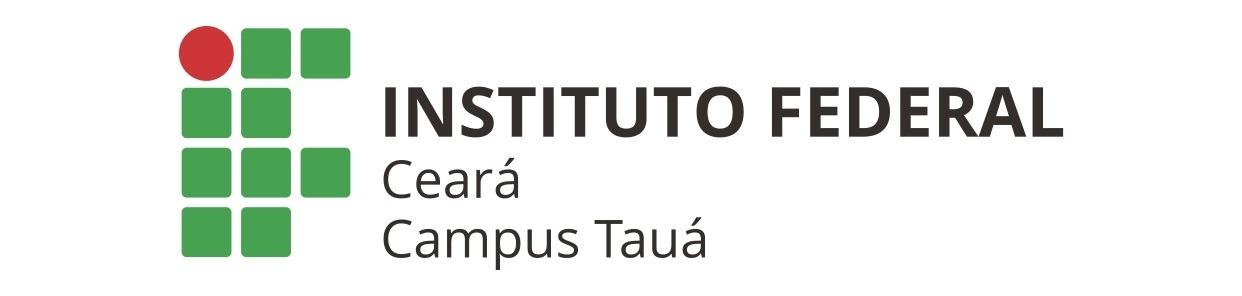
\includegraphics[width=0.65\linewidth]{imgs/logo}
		\end{figure}
		\vspace{-0.8cm}
		\titlepage
	\end{frame}

	\section[Sumário]{}
	
	\begin{frame}
		\frametitle{Sumário}
		%\tableofcontents[hideallsubsections]
		\begin{enumerate}[label=\arabic*.]%[label=\textcolor{black}{\textbullet}]
			\item \reff{introducao}
			\item \reff{fundamentacao}
			%	\begin{enumerate}[label=\alph*.]
			%		\item \reff{fundamentacao-sistemas-posicionamento-interno}
			%		\item \reff{fundamentacao-aprendizado-maquina}
			%		\item \reff{fundamentacao-tecnicas-localizao-indoor}
			%	\end{enumerate}
			\item \reff{trabalhos-relacionados}
			\item \reff{procedimentos}
			\item \reff{resultados-discussoes}
			\item \reff{consideracoes-finais}
			\item \reff{referencias}
		\end{enumerate}
	\end{frame}
	
	\section{Introdução}
	\label{introducao}
	\begin{frame}
		\frametitle{Introdução}
		\begin{itemize}[label=\textcolor{black}{\textbullet}, left=0pt]
			%\setlength\itemsep{10pt}%1em}
			\justifying
			\item {\footnotesize O Sistema de Posicionamento Global (GPS - \textit{Global Positioning System}) é um sistema essencial para a localização em ambientes externos (\textit{outdoor});}
			
			\item {\footnotesize Entretanto, ele possui restrições substanciais de funcionamento em relação a ambientes internos (\textit{indoor});}
			%Isso por conta de bloqueis desses ambientes, ou a interferências que afetam o recebimento das informações via satélite. %Isso pode ocorrer devido a bloqueios por conta da estrutura predial desses ambientes, ou devido à possíveis interferências que afetam o recebimento das informações via satélite, como por exemplo, interferências dos sinais de Wi-Fi (SIMÕES, 2020).
			\item {\footnotesize Uma solução para prover precisão e acurácia em ambientes \textit{indoor}, é a utilização de Sistema de Posicionamento Interno (IPS - \textit{Indoor Positioning System}).}
			%\item Nesse contexto, uma solução que pode prover precisão e acurácia em ambientes \textit{indoor}, é a utilização do Sistema de Posicionamento Interno (IPS - \textit{Indoor Positioning System}).
		\end{itemize}
	\end{frame}

	\begin{frame}
		\frametitle{Introdução}
		\begin{itemize}[label=\textcolor{black}{\textbullet}, left=0pt]
			%\setlength\itemsep{10pt}%1em}
			\justifying
			\item {\footnotesize A tecnologia Wi-Fi é geralmente empregada nos IPSs utilizando o indicador de intensidade do sinal recebido (RSSI - \textit{Received Signal Strength Indicator}), para obter a localização de um nó alvo utilizando a técnica de trilateração, por exemplo.} %aplicada a técnica de trilateração para obter a localização de um nó alvo.
			
			\item {\footnotesize Para obter melhores resultados de localização podem ser utilizadas técnicas baseadas em aprendizado de máquina (\textit{machine learning}), como por exemplo, o \textit{fingerprint}.}
			
			%\item {\footnotesize Diante do exposto, este trabalho se propõe a realizar uma análise da aplicação da técnica de trilateração em conjunto com a técnica de \textit{fingerprint}, como suporte à localização de objetos em sistemas de posicionamento interno, por meio de uma prova de conceito aplicada em um ambiente real.}
			
			%\item Dessa forma, algumas tecnologias empregadas nos sistemas de posicionamento interno são: Banda Ultralarga (UWB - \textit{Ultra Wideband}), Infravermelho, Wi-Fi, \textit{Bluetooth Low Energy} (BLE), Processamento de Imagem, dentre outros (SUN \textit{et al}., 2017).
			
			%\item Além disso, uma forma possível para localizar objetos em ambientes \textit{indoor} é utilizando o indicador de intensidade do sinal recebido (RSSI - \textit{Received Signal Strength Indicator}) dos dispositivos sem fio. Logo, o RSSI é comumente utilizada (facilmente de ser obtido) e encontrada na literatura.
			
			%\item Nesse contexto, o RSSI pode ser aplicado junto com a técnica de trilateração para obter a localização do nó alvo.
		\end{itemize}
		\begin{block}{Objetivo}
			\justifying
			Este trabalho se propõe a realizar uma análise da aplicação da técnica de trilateração em conjunto com a técnica de \textit{fingerprint}, como suporte à localização de objetos em sistemas de posicionamento interno, por meio de uma prova de conceito aplicada em um ambiente real.
		\end{block}
	\end{frame}
	
	\begin{comment}
	\begin{frame}
		\frametitle{Introdução}
		\begin{itemize}[left=0pt]
			\setlength\itemsep{10pt}%1em}
			\justifying
			\item Contudo, somente a técnica de trilateração não provê uma boa precisão e acurácia no processo de localização do nó alvo.
			
			\item Para contornar isso, utiliza-se em conjunto técnicas de aprendizado de máquina (\textit{machine learning}) para ajudar na obtenção de melhores resultados de localização.
			
			\item Existem várias técnicas que podem ser utilizadas em conjunto com a técnicas trilateração, como a técnica de \textit{fingerprint}, por exemplo.
		\end{itemize}
	\end{frame}
	\end{comment}
	
	\begin{comment}
	\begin{frame}
		\frametitle{Fundamentação Teórica}
		\begin{itemize}[left=0pt]
			\setlength\itemsep{10pt}
			\justifying
			\item 
		\end{itemize}		
		%Fundamentação Teórica
	\end{frame}
	\end{comment}
	
	\section{Fundamentação Teórica}
	\label{fundamentacao}
	\subsection{Sistemas de Posicionamento Interno - IPS}
	\label{fundamentacao-sistemas-posicionamento-interno}
	\begin{frame}
		\frametitle{Fundamentação Teórica}
		%\framesubtitle{Sistemas de Posicionamento Interno - IPS}
		\begin{itemize}[label=\textcolor{black}{\textbullet}, left=0pt]
			%\setlength\itemsep{10pt}
			\justifying
			%\item Antes de adentrar a fundo nas técnicas de localização \textit{indoor}, é necessário compreender sobre a estrutura básica e funcionamento dos sistemas de posicionamento interno.
			%\item Segundo Mendes, Lima e Coutinho (2021), as soluções voltadas para posicionamento e navegação em ambientes \textit{indoor} consistem estruturalmente de duas partes: dispositivos móveis e um servidor.
			%\item A arquitetura básica dos sistemas de posicionamento \textit{indoor} consistem estruturalmente de duas partes: dispositivos móveis e um servidor; 
			%\item Essa estrutura pode ser compreendida como a arquitetura básica dos sistemas de posicionamento \textit{indoor}.
			%\item Algumas tecnologias que são utilizadas nos IPSs são: \textit{Bluetooth Low Energy} (BLE), \textit{Wireless Fidelity} (Wi-Fi), \textit{Radio frequency identification} (RFID), Zigbee, dentre outras (MITTELSTADT, 2018).
			\item {\footnotesize Tecnologias utilizadas em IPSs: \textit{Bluetooth Low Energy} (BLE), \textit{Wireless Fidelity} (Wi-Fi), \textit{Radio frequency identification} (RFID), Zigbee, dentre outras (MITTELSTADT, 2018).}
			\begin{block}{Wi-Fi}
				\begin{itemize}[label=\textcolor{black}{\textbullet}, left=5pt]
					\justifying
					\item O Wi-Fi é uma tecnologia amplamente utilizada nos dias atuais, estando presente na maioria dos dispositivos;
					%\item Diferentes estratégias podem ser utilizadas para identificar um local usando Wi-Fi: tempo de chegada do sinal (ToA / TDoA), ângulo de chegada do sinal (AoA) e pela potência de recepção de sinal (RSSI);
					\item Wi-Fi foi muito aceito em sistemas de localização \textit{indoor}.
				\end{itemize}
			\end{block}
			\begin{block}{Aprendizado de Máquina - \textit{Machine Learning}}
				\begin{itemize}[label=\textcolor{black}{\textbullet}, left=5pt]
					\justifying
					\item É um segmento da inteligência artifical (IA) que tem o objetivo de criar algoritmos capazes de construir fluxos lógicos de decisão de forma automatizada; 
					\item Divido em três grupos: supervisionado, não supervisionado e aprendizado por reforço.
				\end{itemize}
			\end{block}
		\end{itemize}
	\end{frame}

	\begin{comment}
	
	\begin{frame}
		\frametitle{Fundamentação Teórica}
		\framesubtitle{Sistemas de Posicionamento Interno - IPS\\ WI-FI}
		\begin{itemize}[left=0pt]
			\setlength\itemsep{10pt}
			\justifying
			\item O WI-FI é uma tecnologia amplamente utilizada nos dias atuais, estando presente na maioria dos dispositivos, como \textit{smartphones}, \textit{tablets}, roteadores, sensores de Internet das coisas (IoT - \textit{Internet of Things}), dentre outros. 
			\item Segundo Simões (2020), diferentes estratégias podem ser utilizadas para identificar um local pelo uso de sinais Wi-Fi, com a utilização de métodos que podem ser baseados no tempo de chegada do sinal (ToA / TDoA), no ângulo de chegada do sinal (AoA) e pela potência de recepção de sinal (RSSI).
			\item Nesse contexto, essa tecnologia foi muito aceita nos sistemas de localização \textit{indoor}, por possuir uma grande quantidade de dispositivos que transmitem Wi-FI, tanto em lugar públicos como privados.
		\end{itemize}
	\end{frame}
	\end{comment}
	
	\begin{comment}
	\subsection{Aprendizado de Máquina - \textit{Machine Learning}}
	\label{fundamentacao-aprendizado-maquina}
	\begin{frame}
		\frametitle{Fundamentação Teórica}
		\framesubtitle{Aprendizado de Máquina - \textit{Machine Learning}}
		\begin{itemize}[label=\textcolor{black}{\textbullet}, left=0pt]
			%\setlength\itemsep{10pt}
			\justifying
			\item O aprendizado de máquina é um segmento da inteligência artificial (IA) que tem como objetivo criar algoritmos capazes de construir fluxos lógicos de decisão de forma automatizada;
			\item Seu uso está associado à possibilidade de soluções para obtenção de informações que não se apresentam de forma clara entre uma grande quantidade de dados (TATSCH, 2019).
			\item Pode ser dividido em três grupos: supervisionado (\textit{supervised learning}), não supervisionado (\textit{unsupervised learning}) e aprendizado por reforço (\textit{reinforcement learning}).
		\end{itemize}		
	\end{frame}
	\end{comment}
	
	\begin{frame}
		\frametitle{Fundamentação Teórica}
		%\framesubtitle{Aprendizado de Máquina - \textit{Machine Learning}}
		\begin{block}{Aprendizado Supervisionado}
			\begin{itemize}[label=\textcolor{black}{\textbullet}, left=5pt]
				%\setlength\itemsep{10pt}
				\justifying
				%\item O aprendizado supervisionado consiste basicamente de algoritmos que mapeiam entradas para saídas desejadas;
				\item O termo supervisionado está relacionado ao fato de que os resultados corretos são conhecidos, servindo assim como um gabarito para o aprendizado do algoritmo;
				\item Consiste basicamente em duas etapas: treino (fase \textit{offline}) e classificação (fase \textit{online});
				%\item Existem vários algoritmos utilizados com esse tipo de aprendizado, por exemplo, \textit{K-Nearest Neighbors} (KNN).
			\end{itemize}
		\end{block}		
		\begin{block}{KNN}
			\begin{itemize}[label=\textcolor{black}{\textbullet}, left=5pt]
				%\setlength\itemsep{10pt}
				\justifying
				\item O KNN é um algoritmo classificador; 
				\item Classifica dados não rotulados de acordo com sua similaridade com classes previamente definidas;
				\item Para a classificação é necessário definir o valor de $K$ vizinhos mais próximos.
			\end{itemize}
		\end{block}	
	\end{frame}

	\begin{comment}
	\begin{frame}
		\frametitle{Fundamentação Teórica}
		\framesubtitle{Aprendizado de Máquina - \textit{Machine Learning}\\ KNN}
		\begin{itemize}[left=0pt]
			\setlength\itemsep{10pt}
			\justifying
			\item O KNN é um algoritmo do tipo classificador, que tem como objetivo classificar dados que não são rotulados de acordo com sua similaridade com classes previamente definidas.
			\item Assim, para realizar a classificação dos dados não rotulados, utiliza-se as informações de $K$ vizinhos mais próximos para classificá-los. 
			\item A definição do parâmetro $K$ é muito importante, pois será ele que determinará a eficácia do modelo. 
		\end{itemize}		
	\end{frame}
	\end{comment}
	
	\subsection{Técnicas de Localização \textit{Indoor}}
	\label{fundamentacao-tecnicas-localizao-indoor}
	\begin{frame}
		\frametitle{Fundamentação Teórica}
		\framesubtitle{Técnicas de Localização \textit{Indoor}}
		\begin{itemize}[label=\textcolor{black}{\textbullet}, left=0pt]
			%\setlength\itemsep{10pt}
			\justifying
			\item {\footnotesize Algumas técnicas utilizadas para a localização em ambientes \textit{indoor}: proximidade, trilateração, triangulação e análise de cena (\textit{fingerprint}) (BERZ, 2015; BARROS, 2016);}
			\item {\footnotesize Essas técnicas podem ser utilizadas em conjunto ou separadamente.} 
		\end{itemize}	
		\begin{block}{Técnica de Trilateração}
			\begin{itemize}[label=\textcolor{black}{\textbullet}, left=5pt]
				%\setlength\itemsep{10pt}
				\justifying
				\item Utilizada para estimar as coordenadas de um determinado objeto a partir de nós de referência previamente conhecidos;
				%\item Utiliza-se o parâmetro RSSI por conta de não necessitar de nenhum \textit{hardware} adicional;
				\item Com o modelo de propagação de sinal log-distância (Equação 1) é possível calcular a distância de dois nós utilizando o RSSI;
				\begin{equation}
					\label{equacao-log-distancia}
					%\hfill 
					P(d) = P_r(d_0) - 10\cdot\beta\cdot\log\left(\frac{d}{d_0}\right)
				\end{equation}
				%\item $P(d)$: sinal recebido em uma distância $d$;
				%\item $P(d_0)$: sinal recebido em uma distância de referência $d_0$ (1 m);
				%\item $\beta$: expoente de perda de caminho (2 a 6).
				%\item Contudo, sua precisão é comprometida por conta de interferências no sinal, além de multi-percurso eventualmente causado por pessoas, objetos ou móveis.
			\end{itemize}
		\end{block}		
	\end{frame}
	
	\begin{comment}
	\begin{frame}
		\frametitle{Fundamentação Teórica}
		\framesubtitle{Técnicas de Localização \textit{Indoor}\\Técnica de Trilateração}
		\begin{itemize}[left=0pt]
			\setlength\itemsep{10pt}
			\justifying
			\item A técnica de trilateração é utilizada para estimar as coordenadas de um determinado objeto a partir de nós de referência que são previamente conhecidos no ambiente (OLIVEIRA, 2021).
			\item Essa técnica consiste na obtenção da localização 2D de um
			dispositivo através da sua distância em relação a três pontos de referência, onde suas posições são conhecidas (SADOWSKI; SPACHOS, 2018).
			\item O parâmetro RSSI é popularmente utilizado nas técnicas de localização \textit{indoor}, por conta de que nenhum adicionado de \textit{hardware} é necessário. 
			\item Entretanto, sua precisão é comprometida por conta de interferências no sinal, além de multi-percurso eventualmente causado por pessoas, objetos ou móveis. 
		\end{itemize}		
	\end{frame}
	\end{comment}
	
	\begin{comment}
	\begin{frame}
		\frametitle{Fundamentação Teórica}
		\framesubtitle{Técnicas de Localização \textit{Indoor}}
		\begin{block}{Técnica de Trilateração}
			\begin{itemize}[label=\textcolor{black}{\textbullet}, left=5pt]
				%\setlength\itemsep{10pt}
				\justifying
				\item A partir do RSSI é possível medir a distância entre dois nós utilizando o modelo log-distância, apresentado na Equação 1. 
				\begin{equation}
					\label{equacao-log-distancia}
					%\hfill 
					P(d) = P_r(d_0) - 10\cdot\beta\cdot\log\left(\frac{d}{d_0}\right)
				\end{equation}
				\item $P(d)$: sinal recebido em uma distância $d$;
				\item $P(d_0)$: sinal recebido em uma distância de referência $d_0$ (1 m);
				\item $\beta$: expoente de perda de caminho (2 a 6).
			\end{itemize}
		\end{block}		
	\end{frame}
	\end{comment}
	
	\begin{comment}
		\begin{itemize}[left=0pt]
		\setlength\itemsep{10pt}
		\justifying
		\item A partir do RSSI é possível medir a distância entre dois nós utilizando o modelo log-distância, apresentado na \hyperlink{equacao-log-distancia}{Equação \autoref{equacao-log-distancia}}.
		\begin{equation}
		\label{equacao-log-distancia}
		%\hfill 
		P(d) = P_r(d_0) - 10\cdot\beta\cdot\log\left(\frac{d}{d_0}\right)
		\end{equation}
		\begin{itemize}[label=\textcolor{black}{\textbullet}]
		\item $P(d)$: sinal recebido em uma distância $d$;
		\item $P(d_0)$: sinal recebido em uma distância de referência $d_0$ (1 m);
		\item $\beta$: expoente de perda de caminho (2 a 6).
		\end{itemize}
		\item A importância de definir o valor de b adequadamente, está na necessidade de buscar uma melhor caracterização do ambiente e canal de propagação do sinal (MENDES; LIMA; COUTINHO, 2021; RAPPAPORT, 2008).
		\end{itemize}
	\end{comment}

	\begin{frame}
		\frametitle{Fundamentação Teórica}
		\framesubtitle{Técnicas de Localização \textit{Indoor} $|$ Técnica de Trilateração}
		
		\begin{figure}
			\caption{Técnica de trilateração para determinar uma posição P}
			\vspace{-5pt}
			\centering
			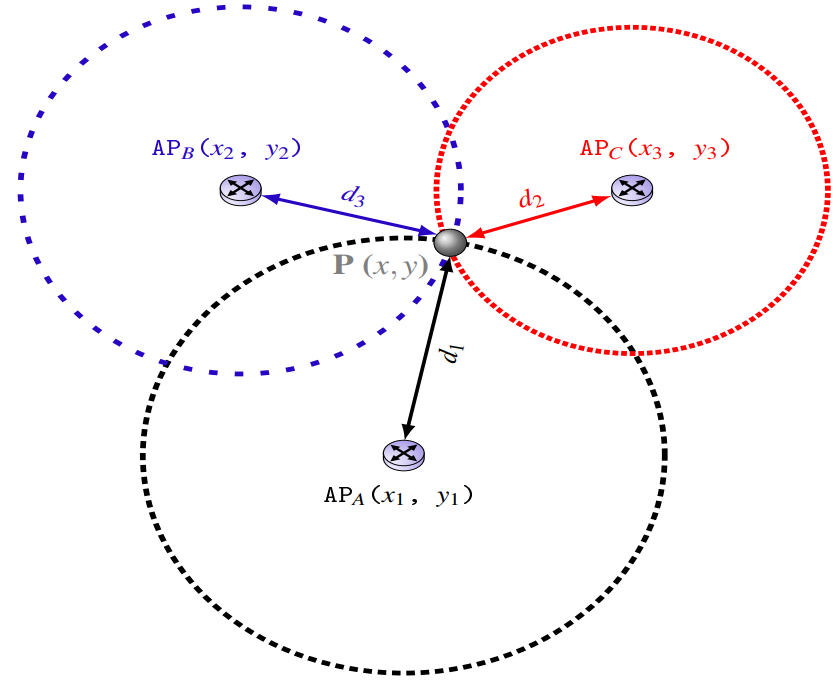
\includegraphics[width=0.65\linewidth]{imgs/trilateracao.PNG}
			\vspace{-5pt}
			\caption*{\tiny{Fonte: Autor (2021).}}
		\end{figure}	
	\end{frame}

	\begin{frame}
		\frametitle{Fundamentação Teórica}
		\framesubtitle{Técnicas de Localização \textit{Indoor}}
		\begin{block}{Técnica de Trilateração}
			\begin{itemize}[label=\textcolor{black}{\textbullet}, left=5pt]
				\justifying
				%\item Com base nas coordenadas de referência: AP$_\text{A}$($x_1$, $y_1$), AP$_\text{B}$($x_2$, $y_2$), e AP$_\text{C}$($x_3$, $y_3$), calcula-se a coordenada da posição desconhecida P($x$, $y$) usando a \hyperlink{equacoes-distancias-trilateracao}{Equação \autoref{equacoes-distancias-trilateracao}}.
				%\begin{equation}
				%	\label{equacoes-distancias-trilateracao}
					%\hfill 
				%	\begin{split}
				%		d_1^2 = (x_1 - x)^2 + (y_1 - y)^2 \\
				%		d_2^2 = (x_2 - x)^2 + (y_2 - y)^2 \\
				%		d_3^2 = (x_3 - x)^2 + (y_3 - y)^2 \\
				%	\end{split}
				%\end{equation}
				\item Sadowski e Spachos (2018), apresentam uma simplificação e redução utilizando o Teorema te Pitágoras para encontrar P($x$, $y$), sendo necessário posicionar os APs no seguinte padrão: AP$_\text{A}$($0$, $0$), AP$_\text{B}$($p$, $0$), e AP$_\text{C}$($q$, $r$). %As coordenadas de $x$, $y$ são apresentadas nas Equações 3 e 4.
			\end{itemize}
			\begin{equation}
				\label{equacoes-simplificada-trilateracao-x}
				x = \frac{d_1^2-d_2^2+p^2}{2\cdot p}
			\end{equation}
			\begin{equation}
				\label{equacoes-simplificada-trilateracao-y}
				y = \frac{d_1^2-d_3^2+q^2+r^2}{2\cdot r} - x\cdot\frac{q}{r}
			\end{equation}		
		\end{block}
		\begin{block}{Técnica de \textit{Fingerprint}}
			\begin{itemize}[label=\textcolor{black}{\textbullet}, left=5pt]
				\justifying
				%\item A técnica de \textit{fingerprint} é uma técnica que utiliza um infraestrutura de redes sem fio em ambientes \textit{indoor} ou em locais que o GPS não funciona corretamente; %ou em outros locais onde o sistema GPS não funciona corretamente (KHALEL, 2010).
				\item Consiste de duas epatas: treinamento (fase \textit{offline}) e localização (fase \textit{online}).
				\item Utiliza-se o aprendizado supervisionado, visto que realiza-se as fases de treinamento (\textit{offline}) e classificação (\textit{online});
				%\item Assim, utilizou-se o algoritmo KNN, por ser muito encontrado na literatura e ser simples a sua implementação.
			\end{itemize}
		\end{block}
	\end{frame}

	\begin{comment}
		\begin{frame}
			\frametitle{Fundamentação Teórica}
			\framesubtitle{Técnicas de Localização \textit{Indoor}}
			\begin{block}{Técnica de \textit{Fingerprint}}
				\begin{itemize}[label=\textcolor{black}{\textbullet}, left=5pt]
					\justifying
					%\item A técnica de \textit{fingerprint} é uma técnica que utiliza um infraestrutura de redes sem fio em ambientes \textit{indoor} ou em locais que o GPS não funciona corretamente; %ou em outros locais onde o sistema GPS não funciona corretamente (KHALEL, 2010).
					\item Consiste de duas epatas: treinamento (fase \textit{offline}) e localização (fase \textit{online}).
					\item Utiliza-se o aprendizado supervisionado, visto que realiza-se as fases de treinamento (\textit{offline}) e classificação (\textit{online});
					\item Assim, utilizou-se o algoritmo KNN, por ser muito encontrado na literatura e ser simples a sua implementação.
				\end{itemize}
			\end{block}
		\end{frame}
	\end{comment}
	%\captionsetup{justification=raggedright,singlelinecheck=false}
	\renewcommand{\arraystretch}{1.4}
	\addtolength{\tabcolsep}{1.5pt}
	
	
	\section{Trabalhos Relacionados}
	\label{trabalhos-relacionados}
	\begin{frame}
		\frametitle{Trabalhos Relacionados}
		\begin{table}[]
			\centering
			\caption*{Quadro 1: Resumo trabalhos relacionados}
			\label{tabela-trabalhos-relacionados}
			\vspace{-15pt}
			\resizebox{\columnwidth}{!}{%
			\begin{tabular}{|c|c|c|}
				\hline
				\textbf{Autores} & \textbf{Titulo} & \textbf{Tecnologias e Técnicas} \\ \hline
				Aravena e Delzari (2021) & \begin{tabular}[c]{@{}c@{}}Desenvolvimento de aplicativo para auxílio\\ à navegação em ambientes internos\end{tabular} & \begin{tabular}[c]{@{}c@{}}Android; Wi-Fi;\\ RSSI; Centroide; \\ Centróide ponderado; \\ Trilateração;\end{tabular} \\ \hline
				Moreira, Farias e Carvalho (2017) & \begin{tabular}[c]{@{}c@{}}Posicionamento em Ambientes Internos com\\ Dispositivos Wi-Fi de Baixo Custo\end{tabular} & \begin{tabular}[c]{@{}c@{}}ESP8266; Wi-Fi; \\ RSSI; Trilateração;\end{tabular} \\ \hline
				Weerasinghe e Dissanayake (2019) & \textit{\begin{tabular}[c]{@{}c@{}}Towards IoT; Comparison of RSS based \\ indoor localization using supervised \\ learning and trilateration in WSN\end{tabular}} & \begin{tabular}[c]{@{}c@{}}Rede Neural Artificial; \\ ESP8266; Wi-Fi; RSSI; \\ Trilateração; MQTT;\end{tabular} \\ \hline
				Mari, Kiong e Kim (2018) & \textit{\begin{tabular}[c]{@{}c@{}}A hybrid trilateration and fingerprinting \\ approach for indoor localization base on wifi\end{tabular}} & \begin{tabular}[c]{@{}c@{}}Wi-Fi; RSSI; Trilateração; \\ \textit{fingerprint}; KOS-ELM;\end{tabular} \\ \hline
			\end{tabular}}
			\vspace{-5pt}
			\caption*{\tiny{Fonte: Autor (2021).}}
		\end{table}
	\end{frame}
	
	\section{Procedimentos Metodológicos}
	\label{procedimentos}
	\begin{frame}
		\frametitle{Procedimentos Metodológicos}
		%\begin{itemize}[label=\textcolor{black}{\textbullet}, left=0pt]
		%	\justifying
			%\item {\footnotesize Este trabalho se propôs a realizar uma análise da aplicação da técnica trilateração em conjunto com a técnica de \textit{fingerprint}, como suporte à localização de objetos em IPS;}
		%	\item {\footnotesize Realizou-se uma Revisão Sistemática da Literatura (RSL);}
			%\item \textit{(``machine learning'' OR ``supervised learning'' OR ``unsupervised learning'' OR ``neural network'' OR ``reinforcement learning") AND (``Wi-Fi based localization'' OR ``trilateration technique'' OR ``trilateration'' OR ``wireless based localization'') AND (``indoor location'' OR ``indoor localization'') AND (IPS OR ``indoor navigation'' OR ``indoor positioning system'' OR ``indoor positioning'')}.
		%\end{itemize}	
		\begin{block}{Projeto de Experimento}
			\begin{itemize}[label=\textcolor{black}{\textbullet}, left=5pt]
				\justifying
				%\item Este trabalho se propôs a realizar uma análise da aplicação da técnica trilateração em conjunto com a técnica de \textit{fingerprint}, como suporte à localização de objetos em IPS;
				%\item Utilizou-se o parâmetro RSSI em redes sem fio Wi-Fi;
				\item Realizou-se uma Revisão Sistemática da Literatura (RSL);
				\item Utilizou-se a tecnologia Wi-Fi como o parâmetro RSSI;
				%\item Técnica de análise utilizada foi a medição (metros);
				%\item Métricas de desempenho utilizadas: erro médio absoluto (MAE) e raiz quadrática média dos erros (RMSE);
				\item Nó sensor de captura do RSSI utilizado: \textit{smartphone} modelo Redmi Note 9S;
				\item Nós de referência utilizados: três roteadores modelo RE163 (1,25 m do piso);
				\item Para o \textit{fingerprint} utilizou-se o algoritmo KNN para treinar e testar o modelo de classificação, implementado em Python utilizando a biblioteca \textit{scikit-learn};
				\item Para a trilateração aplicou-se o modelo log-distância utilizando a linguagem Python com a biblioteca \textit{pandas} para manipulação dos dados.
			\end{itemize}
		\end{block}
	\end{frame}

	\begin{comment}
	\begin{frame}
		\frametitle{Procedimentos Metodológicos}	
		\begin{block}{Projeto de Experimento}
			\begin{itemize}[label=\textcolor{black}{\textbullet}, left=5pt]
				\justifying
				%\item Este trabalho se propôs a realizar uma análise da aplicação da técnica trilateração em conjunto com a técnica de \textit{fingerprint}, como suporte à localização de objetos em IPS;
				\item Utilizou-se o parâmetro RSSI em redes sem fio Wi-Fi;
				\item Técnica de análise utilizada foi a medição (metros);
				\item Métricas de desempenho utilizadas: erro médio absoluto (MAE) e raiz quadrática média dos erros (RMSE).
				\item O nó sensor para a captura do RSSI utilizado foi um \textit{smartphone} modelo Redmi Note 9S;
				\item Utilizou-se três roteadores modelo RE163 como nós de referência (APs), posicionados a 1,25 m do piso;
				\item Para o \textit{fingerprint} utilizou-se o algoritmo KNN para treinar e testar o modelo de classificação, implementado em Python utilizando a biblioteca \textit{scikit-learn};
				\item Para a trilateração aplicou-se o modelo log-distância utilizando a linguagem Python com a biblioteca \textit{pandas} para manipulação dos dados.
			\end{itemize}
		\end{block}
	\end{frame}
	\end{comment}
	%\captionsetup{justification=raggedright,singlelinecheck=false}
	
	\begin{frame}
		\frametitle{Procedimentos Metodológicos}	
		\begin{block}{Ambiente de Aplicação}
			\begin{itemize}[label=\textcolor{black}{\textbullet}, left=5pt]
				\justifying
				\item Ambiente de aplicação foi uma sala de aula do IFCE - \textit{Campus} Tauá;
				\item Dimensões adotadas para o experimento: 8 m (L) $\times$ 6 m (C), uma área de 48 m$^2$;
				\item Para o \textit{fingerprint} dividiu-se a sala em 12 regiões de 4 m$^2$ (numeradas de 1 a 12);
				\item Coordenadas dos APs (em metros), em relação à área delimitada para o experimento: AP$_\text{A}$ ($0.17$, $0$), AP$_\text{B}$ ($5.83$, $0$), AP$_\text{C}$ ($3.30$, $7.90$);
				\item Coordenadas dos APs para a trilateração: AP$_\text{A}$ ($0$, $0$), AP$_\text{B}$ ($5.66$, $0$), AP$_\text{C}$ ($3.13$, $7.90$);
				\item As coordenadas das aplicações de teste são apresentadas na Tabela 1.
				%\item As coordenadas de aplicação dos testes de trilateração são apresentadas na Tabela 1.%, foram escolhidas quatros regiões ao acaso e dois pontos ao acaso de cada região, além do centro de cada região.
			\end{itemize}
		\end{block}
		\begin{figure}
			\caption*{Tabela 1: Coordenadas das posições de coleta}
			\vspace{-5pt}
			\centering
			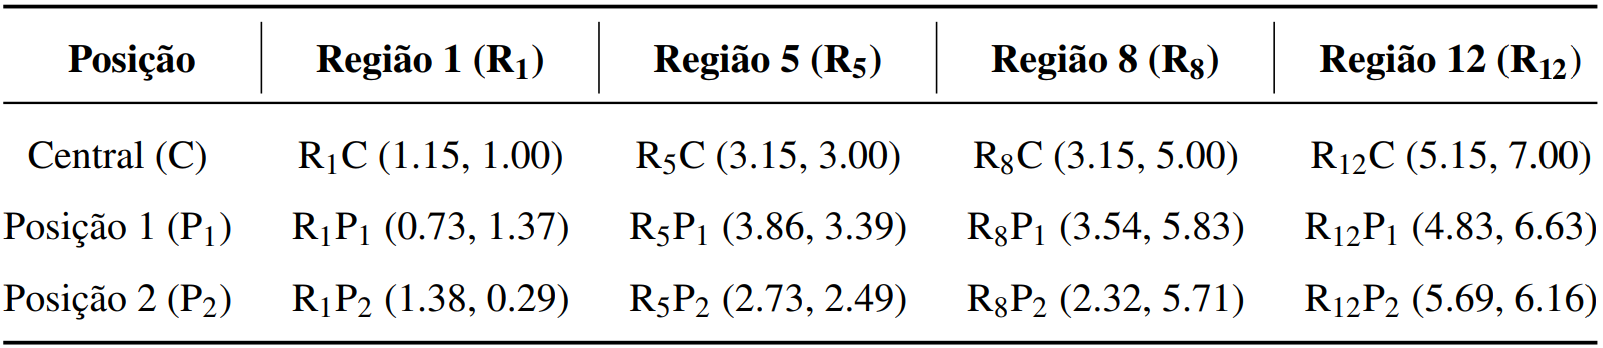
\includegraphics[width=0.78\linewidth]{imgs/tabela_regioes.PNG}
			\vspace{-5pt}
			\caption*{\tiny{Fonte: Autor (2021).}}
		\end{figure}
	\end{frame}

	\begin{frame}
		\frametitle{Procedimentos Metodológicos}	
		\begin{figure}
			\caption{Divisão das regiões e disposição dos APs}
			\vspace{-5pt}
			\centering
			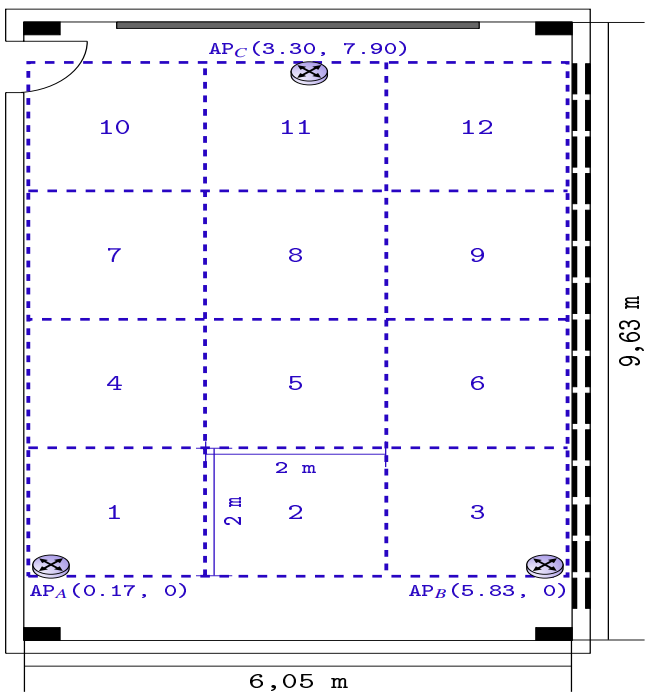
\includegraphics[width=0.55\linewidth]{imgs/mapeamento.PNG}
			\vspace{-5pt}
			\caption*{\tiny{Fonte: Autor (2021).}}
		\end{figure}
	\end{frame}

	\begin{frame}
		\frametitle{Procedimentos Metodológicos}	
		\begin{block}{Condução do Experimento}
			\begin{itemize}[label=\textcolor{black}{\textbullet}, left=5pt]
				\justifying
				\item Para o mapeamento do \textit{fingerprint} (fase \textit{offline}), realizou-se no período da tarde a captura dos RSSIs em cada centro de região (60 medições);
				%\item Para o mapeamento do \textit{fingerprint} (fase \textit{offline}), realizou-se em cada região no período da tarde, a captura dos RSSIs em cada centro de região, realizado 60 medições;
				\item Desenvolveu-se um aplicativo para facilitar e automatizar a coleta dos dados, configurando alguns parâmetros;%, desenvolveu um aplicativo %multi-plataforma, sendo possível definir alguns parâmetros para a coleta;
				%\item Para evitar as interferências do aplicador, o aplicativo é configurado com um tempo de guarda antes da leitura;
				%\item Ao fim da coleta todos os dados e parâmetros são armazenados em um arquivo csv;
				\item Ao término da fase \textit{offline} obteve-se um total de 720 medições, armazenadas em um único arquivo csv, onde realizou-se um processo de normalização dos dados;% substituindo os valores de \textit{outliers} coletados pela média aritmética dos respectivos dados.
				%\item Após a normalização realizou-se o treinamento do modelo de classificação utilizando o KNN, onde o melhor valor de $K$ foi escolhido com base em diversos valores treinados.
				\item Em seguida, realizou-se o treinamento do modelo de classificação utilizando o KNN, usando um valor de $K=26$;
				\item Após a fase \textit{offline}, obteve-se os valores de $\beta$ (coeficiente de perda de percurso) para cada região do \textit{fingerprint} para ser aplicado na técnica de trilateração.
				%\item O valor de $\beta$ encontrado é o ideal para cada AP naquela região.
				%\item Valores fora do intervalo de 2 a 6 foram substituídos para os valores mais próximos, como segure Rappaport (2008).
			\end{itemize}
		\end{block}
	\end{frame}

	\begin{comment}
		\begin{frame}
			\frametitle{Procedimentos Metodológicos}	
			\begin{block}{Condução do Experimento}
				\begin{itemize}[label=\textcolor{black}{\textbullet}, left=5pt]
					\justifying
					%\item Para o mapeamento do \textit{fingerprint} (fase \textit{offline}), realizou-se em cada região no período da tarde, a captura dos RSSIs em cada centro de região, realizado 60 medições;
					%\item Para facilitar e automatizar a coleta dos dados, desenvolveu um aplicativo multi-plataforma, sendo possível definir alguns parâmetros para a coleta;
					%\item Para evitar as interferências do aplicador, o aplicativo é configurado com um tempo de guarda antes da leitura;
					%\item Ao fim da coleta todos os dados e parâmetros são armazenados em um arquivo csv;
					%\item Ao término da fase \textit{offline} obteve-se um total de 720 medições, sendo armazenadas em um único csv;
					%\item Em seguida, realizou-se um processo de normalização dos dados, substituindo os valores de \textit{outliers} coletados pela média aritmética dos respectivos dados;
					%\item Após a normalização realizou-se o treinamento do modelo de classificação utilizando o KNN, onde o melhor valor de $K$ foi escolhido com base em diversos valores treinados, utilizando $K=26$;
					\item Em seguida, realizou-se o treinamento do modelo de classificação utilizando o KNN, usando um valor de $K=26$;
					\item Após a fase \textit{offline}, obteve-se os valores de $\beta$ (coeficiente de perda de percurso) para cada região do \textit{fingerprint} para ser aplicado na técnica de trilateração;
					\item Os valores de $\beta$ foram obtidos com base na média dos RSSI de cada AP em cada região;%, calculando a distância do centro da região para cada AP e utilizando no modelo log-distância;
					\item O valor de $\beta$ encontrado é o ideal para cada AP naquela região; 
					\item Valores fora do intervalo de 2 a 6 foram substituídos para os valores mais próximos, como segure Rappaport (2008).
				\end{itemize}
			\end{block}
		\end{frame}
	\end{comment}
	\begin{frame}
		\frametitle{Procedimentos Metodológicos}
		\begin{figure}
			\caption{Aplicativo desenvolvido para a captura dos RSSIs}
			\vspace{-5pt}
			\centering
			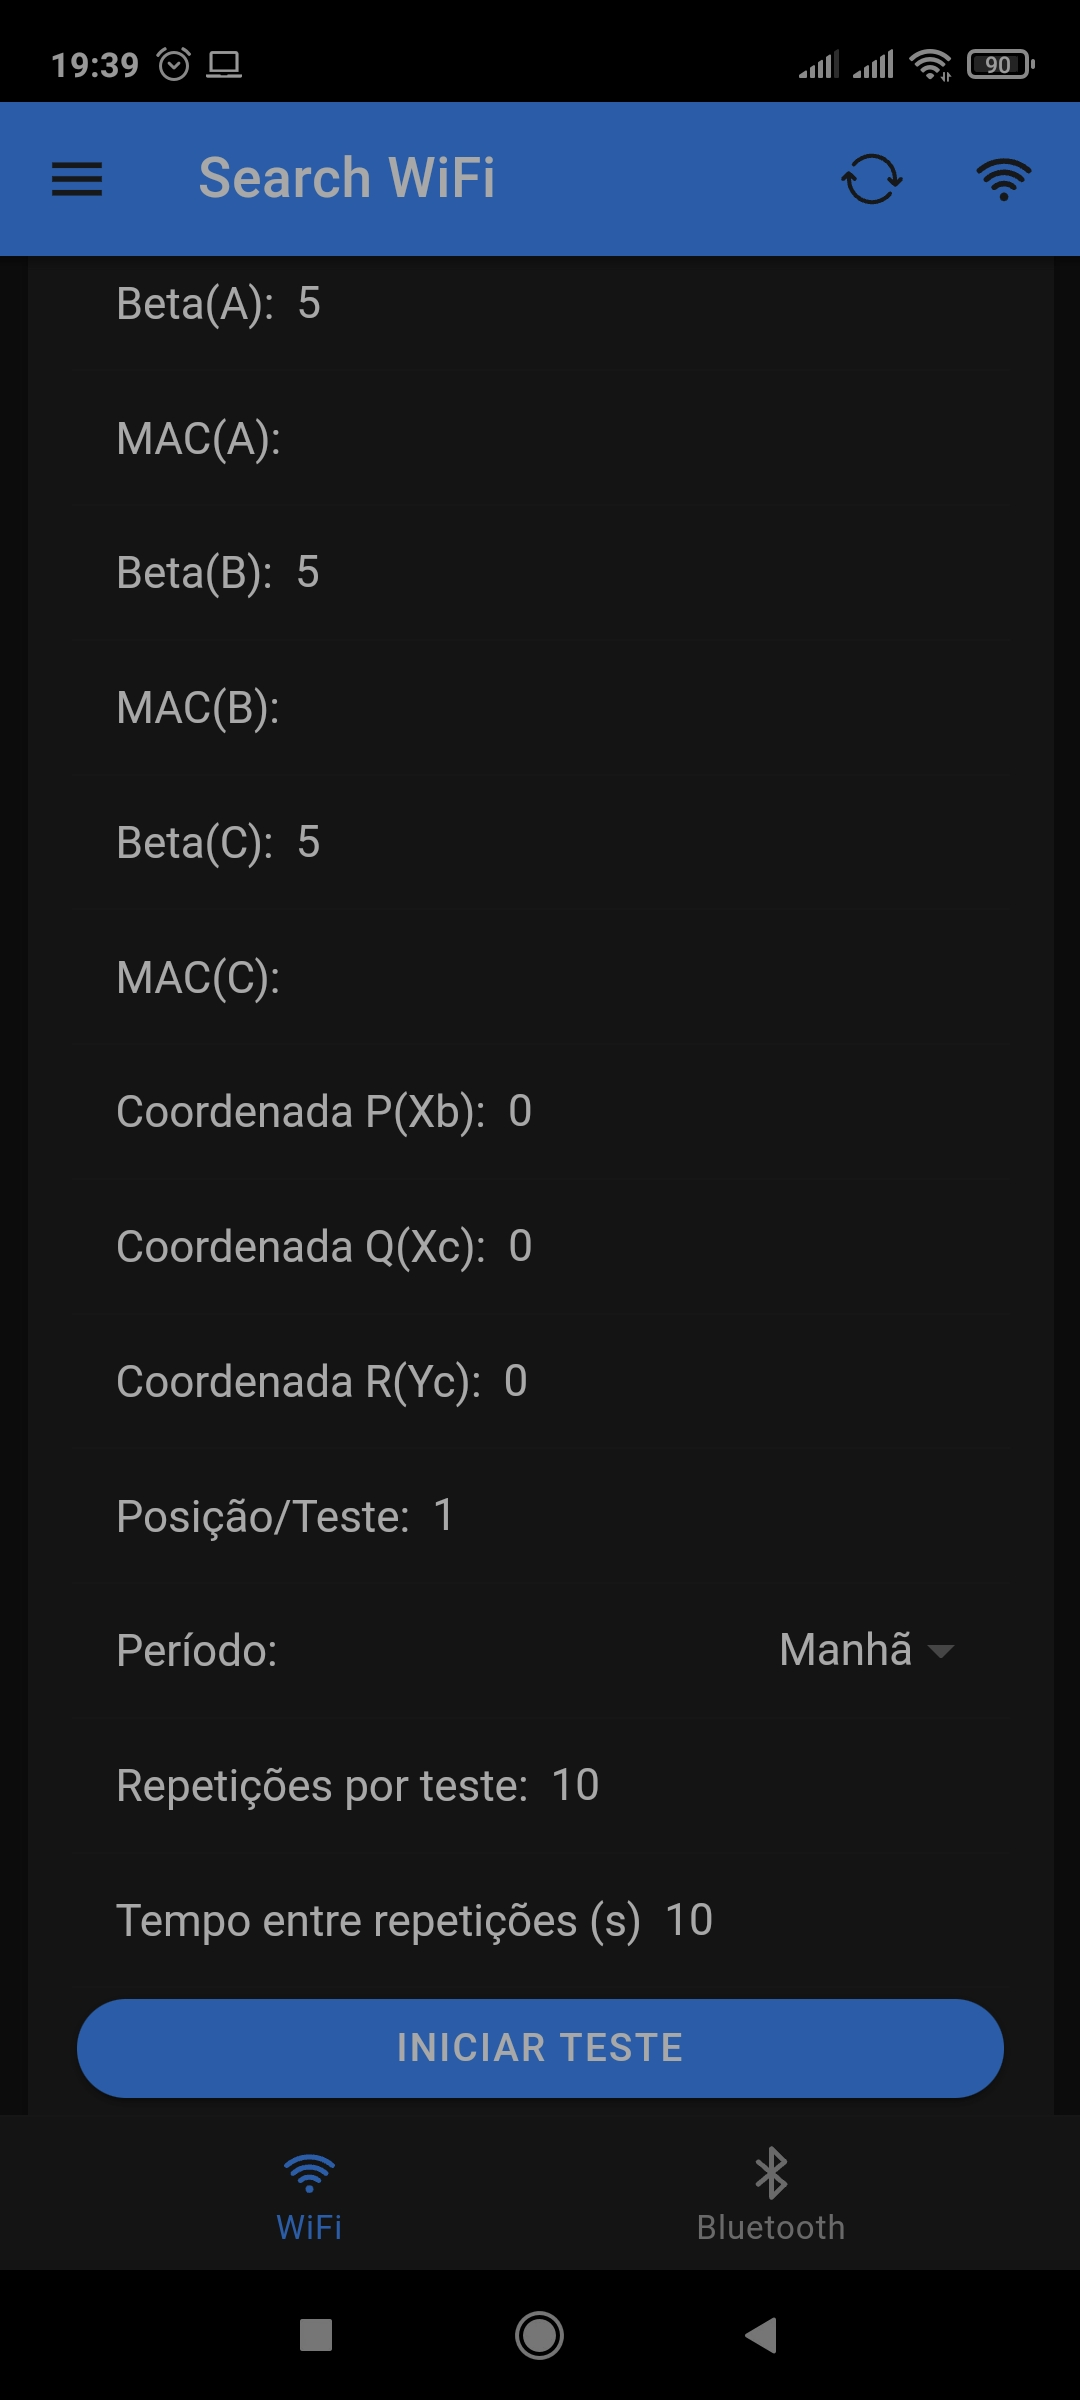
\includegraphics[width=5cm, height=6.9cm]{imgs/app_1.jpg}
			\vspace{-5pt}
			\caption*{\tiny{Fonte: Autor (2021).}}
		\end{figure}
	\end{frame}

	\begin{frame}
		\frametitle{Procedimentos Metodológicos}	
		\begin{block}{Condução do Experimento}
			\begin{itemize}[label=\textcolor{black}{\textbullet}, left=5pt]
				\justifying
				\item Para a fase \textit{online}, realizou-se as medições de acordo com as coordenadas de testes apresentados na Tabela 1;% dos centros das quatro regiões, escolhias para os testes, e os dois pontos, apresentados na Tabela 1.
				\item As coletas de teste foram realizadas em três períodos distintos: manhã, tarde, e noite;
				\item Para cada bateria foram realizadas 20 medições de RSSI em intervalos de 10 s;
				\item Ao término da fase \textit{online} obteve-se um total de 720 medições, sendo armazenadas em três arquivos csv;%, separados por período de captura, realizando o mesmo procedimento de normalização dos dados;
				%\item Realizou-se nessa fase o mesmo procedimento de normalização dos dados realizado na fase \textit{offline};
				\item Os dados de teste foram submetidos ao modelo treinado, onde o KNN realizou o processo de predição dos dados, retornando a região classificada;
				%\item Em seguida, as instâncias de dados não rotuladas foram submetidas ao modelo treinado, onde o classificador KNN realizou o processo de predição dos dados, retornando a região de cada nova instância;
				\item Comparou-se os dados retornados com as regiões reais e aplicou-se o valor $\beta$ a cada AP na técnica de trilateração.
				%\item Essas instâncias determinadas foram comparadas com as regiões reais para uma análise e aplicou-se o valor de $\beta$ a cada AP na técnica de trilateração.
			\end{itemize}
		\end{block}
	\end{frame}%COPIA COM ALGUMAS CORREÇÕES PARA FAZER
	
	\section{Resultados e Discussões}
	\label{resultados-discussoes}
	\begin{frame}
		\frametitle{Resultados e Discussões}
		\framesubtitle{Aplicação da Técnica de \textit{Fingerprint}}
		\begin{figure}
			\caption{Média e desvio padrão de RSSI para cada AP em cada região}
			\vspace{-5pt}
			\centering
			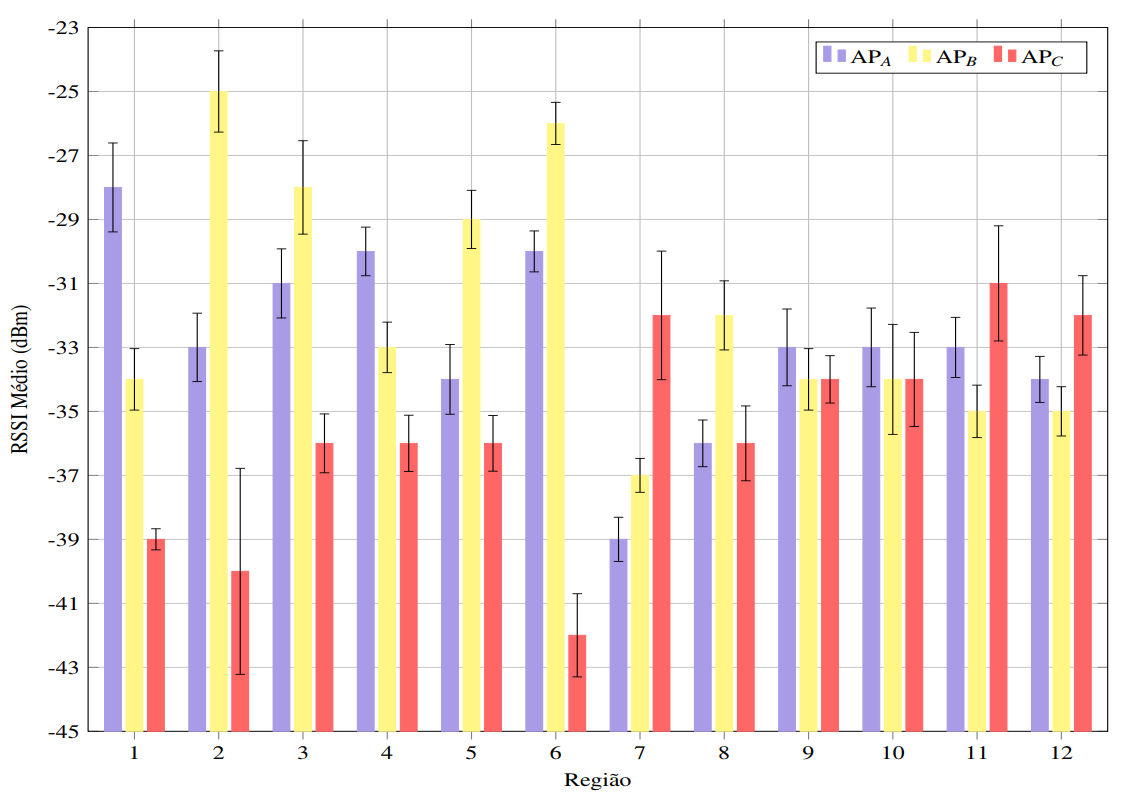
\includegraphics[width=12cm, height=6.2cm]{imgs/grafico_rssi.PNG}
			\vspace{-12pt}
			\caption*{\tiny{Fonte: Autor (2021).}}
		\end{figure}
	\end{frame}
	
	\begin{frame}
		\frametitle{Resultados e Discussões}
		\begin{block}{Aplicação da Técnica de \textit{Fingerprint}}
			\begin{itemize}[label=\textcolor{black}{\textbullet}, left=5pt]
				\justifying
				\item Para a técnica do \textit{fingerprint}, obteve-se 57,36\% de acurácia geral na classificação correta das regiões, para todos os pontos em todos os períodos;
				\item A região que apresentou a maior acurácia foi a região 1 (91,67\%) e a com menor acurácia foi região 5 (42,22\%);
				%\item A região que apresentou a menor acurácia foi a região 5 (42,22\%);
				\item Entretanto, a região 5 obteve-se classificações de regiões próximas, sendo as regiões 4 (16,11\%) e 8 (15\%) suas vizinhas do lado esquerdo e acima, respectivamente.
				%\item As regiões 8 e 12, obtiveram uma boa acurácia de classificação, porém a maioria das classificações incorretas foram em regiões distantes.% o que pode prejudicar a aplicação futura da técnica de trilateração.
			\end{itemize}
		\end{block}
	\end{frame}
	
	\begin{frame}
		\frametitle{Resultados e Discussões}
		\framesubtitle{Aplicação da Técnica de \textit{Fingerprint}}
		\begin{figure}
			\caption{Matriz de confusão da técnica de \textit{fingerprint} para todos os pontos}
			\vspace{-5pt}
			\centering
			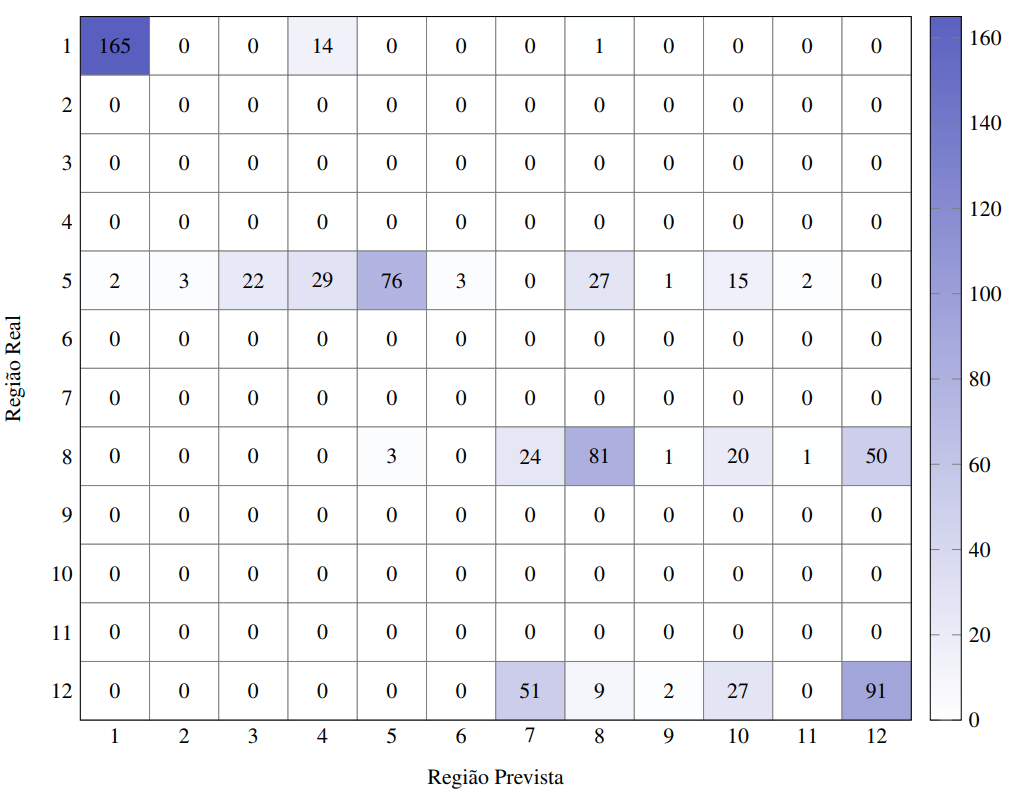
\includegraphics[width=10cm, height=6.4cm]{imgs/matrix_confusao.PNG}
			\vspace{-5pt}
			\caption*{\tiny{Fonte: Autor (2021).}}
		\end{figure}
	\end{frame}
	
	\begin{frame}
		\frametitle{Resultados e Discussões}
		\framesubtitle{Aplicação da Técnica de \textit{Fingerprint}}
		\begin{block}{}
			\begin{itemize}[left=0pt]%[label=\textcolor{black}{\textbullet}]
				\justifying
				\item Com o modelo treinado obteve-se as seguintes taxas de acurácia em cada período individualmente: 53,33\% pela manhã, 54,16\% pela tarde e 64,58\% pela noite.
			\end{itemize}
		\end{block}
		\begin{figure}
			\caption*{Tabela 2: Acurácia de classificação por período}
			\vspace{-5pt}
			\centering
			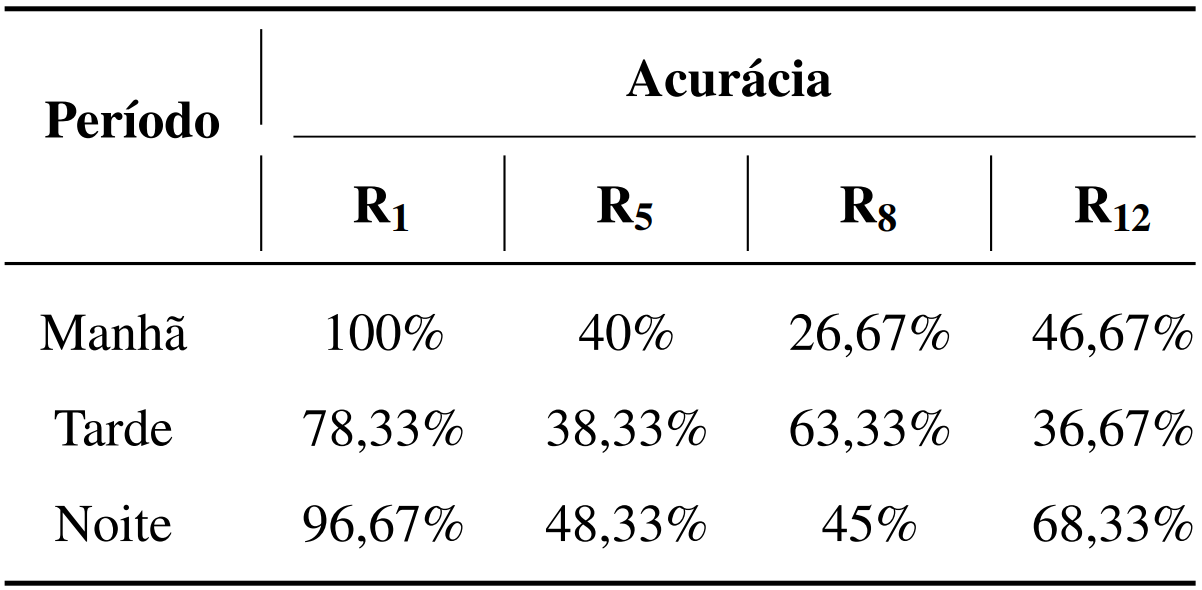
\includegraphics[width=7.5cm, height=3.5cm]{imgs/tabela_acuracia_por_periodo.PNG}
			\vspace{-5pt}
			\caption*{\tiny{Fonte: Autor (2021).}}
		\end{figure}
	\end{frame}
	
	\begin{frame}
		\frametitle{Resultados e Discussões}
		\framesubtitle{Aplicação da Técnica de Trilateração}
		%\begin{block}{}
		%	\begin{itemize}[left=0pt]%[label=\textcolor{black}{\textbullet}]
		%		\justifying
		%		\item Após a fase \textit{offline} da técnica de \textit{fingerprint}, foram obtidos os valores de $\beta$ de forma experimental para cada AP em cada região mapeada. % Esses valores foram obtidos de forma experimental com base na equação do modelo log-distância.
		%	\end{itemize}
		%\end{block}
		\begin{figure}
			\caption*{Tabela 3: Valores do fator de perda de percurso ($\beta$) em cada centro de região para cada AP}
			\vspace{-5pt}
			\centering
			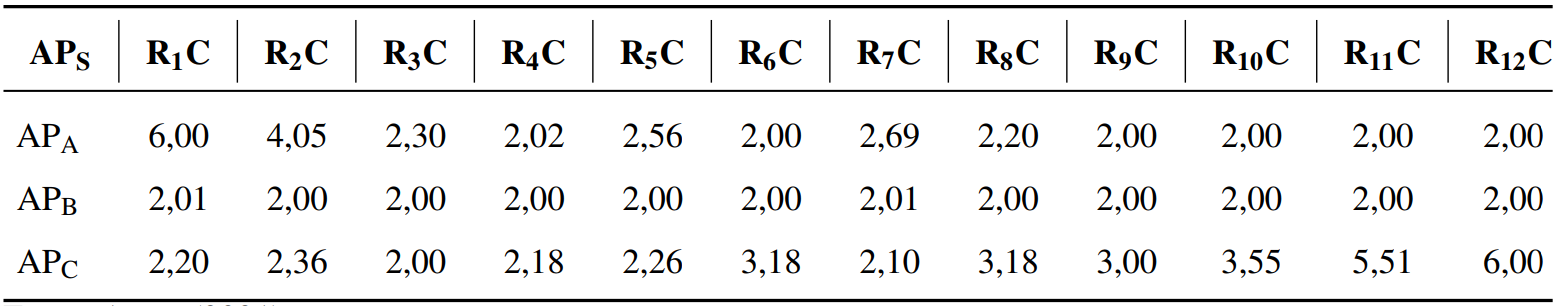
\includegraphics[width=10.5cm, height=3cm]{imgs/betas.PNG}
			\vspace{-5pt}
			\caption*{\tiny{Fonte: Autor (2021).}}
		\end{figure}
	\end{frame}

	\begin{frame}
		\frametitle{Resultados e Discussões}
		%\framesubtitle{Aplicação da Técnica de Trilateração}
		\begin{block}{Aplicação da Técnica de Trilateração}
			\begin{itemize}[label=\textcolor{black}{\textbullet}, left=5pt]
				\justifying
				%\item Dessa forma, foi possível calcular a posição estimada com base na média dos valores RSSI;% coletados de cada AP em cada posição de teste escolhida (fase online);
				\item Para definir a posição estimada pela trilateração, utilizou-se os valores de $\beta$ com base na região classificada pelo modelo treinado na aplicação do \textit{fingerprint};
				\item Para ajustar a posição estimada no método de trilateração, foram utilizados dois métodos de ajuste:
				\begin{enumerate}[label=\arabic*.]
					\item Deslocamento para a região classificada no \textit{fingerprint}, desde que obtido 75\% de taxa de classificação em uma mesma região;
					\item Combinação das posições estimadas com base nas duas regiões de maior taxa de classificação pelo modelo (se a taxa de classificação $<$ 75\%);%em uma mesma região for menor que 75\%.
				\end{enumerate}
			\end{itemize}
		\end{block}
	\end{frame}

	\begin{frame}
		\frametitle{Resultados e Discussões}	
		\begin{figure}
			\caption*{Figura 6: Divisão das regiões e disposição dos APs}
			\vspace{-5pt}
			\centering
			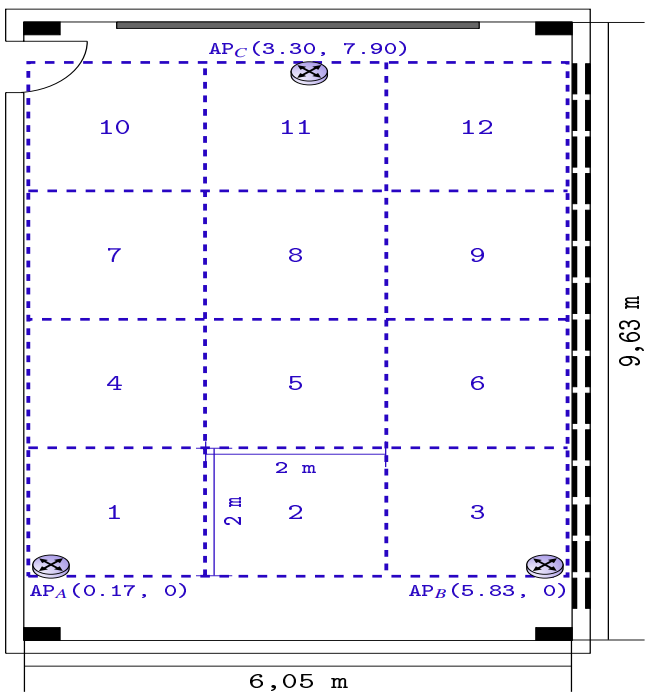
\includegraphics[width=0.55\linewidth]{imgs/mapeamento.PNG}
			\vspace{-5pt}
			\caption*{\tiny{Fonte: Autor (2021).}}
		\end{figure}
	\end{frame}

	\begin{frame}
		\frametitle{Resultados e Discussões}
		\framesubtitle{Aplicação da Técnica de Trilateração}
		\begin{figure}
			\caption*{Figura 7: Posições estimadas no período da manhã}
			\vspace{-5pt}
			\centering
			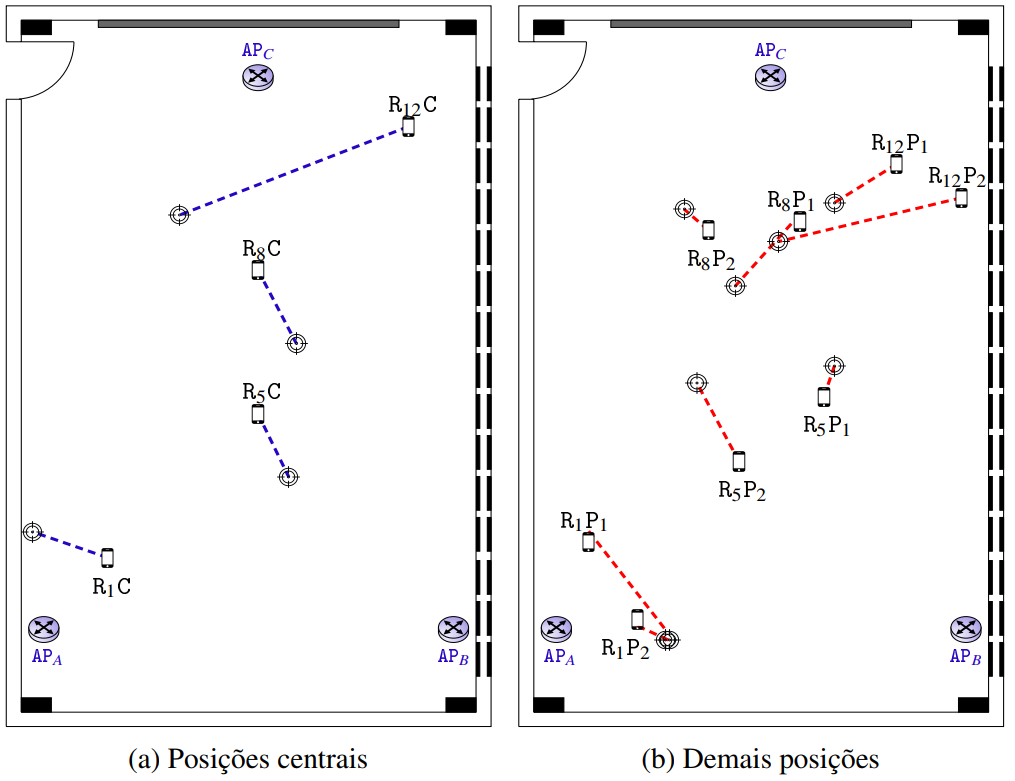
\includegraphics[width=8.5cm, height=6.5cm]{imgs/manha.PNG}
			\vspace{-5pt}
			\caption*{\tiny{Fonte: Autor (2021).}}
		\end{figure}
	\end{frame}

	\begin{frame}
		\frametitle{Resultados e Discussões}
		\framesubtitle{Aplicação da Técnica de Trilateração}
		\begin{figure}
			\caption*{Figura 8: Posições estimadas no período da tarde}
			\vspace{-5pt}
			\centering
			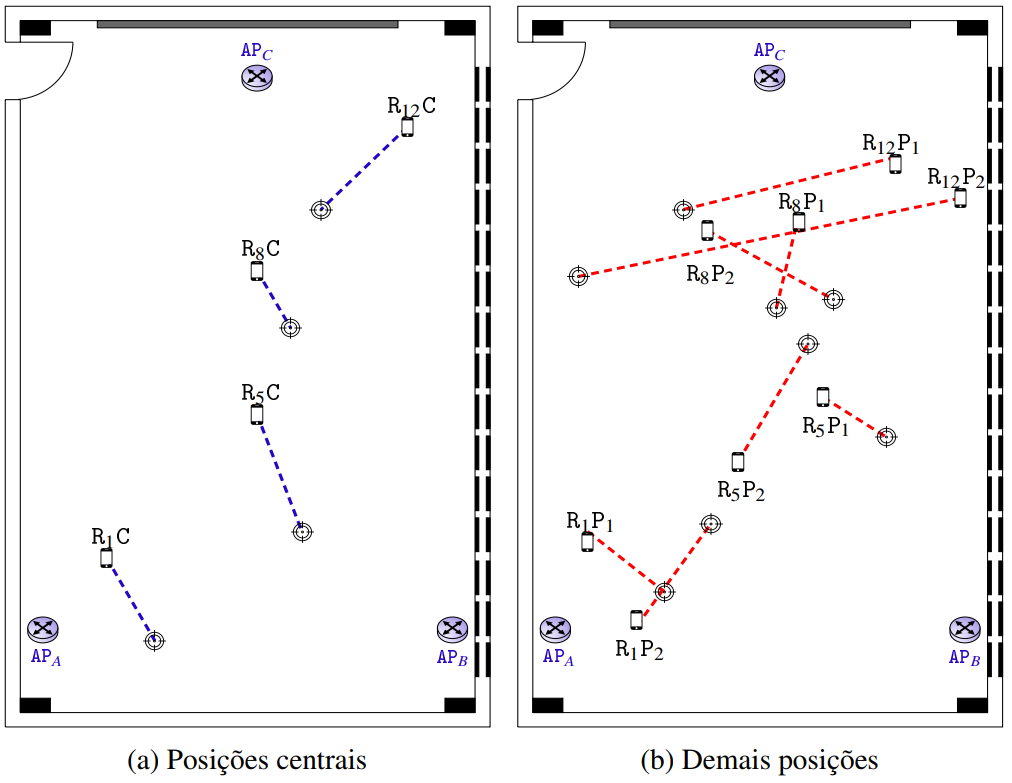
\includegraphics[width=8.5cm, height=6.5cm]{imgs/tarde.PNG}
			\vspace{-5pt}
			\caption*{\tiny{Fonte: Autor (2021).}}
		\end{figure}
	\end{frame}

	\begin{frame}
		\frametitle{Resultados e Discussões}
		\framesubtitle{Aplicação da Técnica de Trilateração}
		\begin{figure}
			\caption*{Figura 9: Posições estimadas no período da noite}
			\vspace{-5pt}
			\centering
			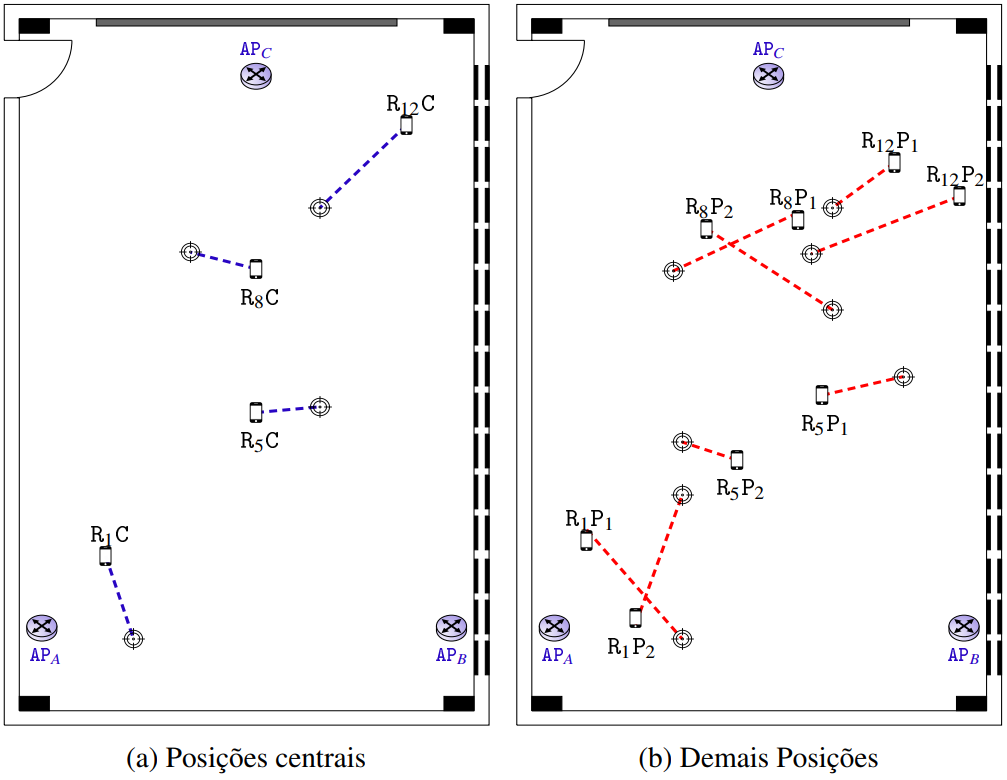
\includegraphics[width=8.5cm, height=6.5cm]{imgs/noite.PNG}
			\vspace{-5pt}
			\caption*{\tiny{Fonte: Autor (2021).}}
		\end{figure}
	\end{frame}

	\begin{frame}
		\frametitle{Resultados e Discussões}
		%\framesubtitle{Aplicação da Técnica de Trilateração}
		\begin{block}{Aplicação da Técnica de Trilateração}
			\begin{itemize}[label=\textcolor{black}{\textbullet}, left=5pt]
				\justifying
				\item As métricas utilizadas para avaliar o desempenho das técnicas, em função do erro de localização, foram: erro médio absoluto (MAE) e raiz quadrática média dos erros (RMSE).
				%\item A MAE é utilizada para encontrar o erro médio absoluto em cada AP nas posições de testes;
				%\item O RMSE é utilizado para calcular a raiz do erro médio quadrático entre a posição real e a posição estimada.
				
			\end{itemize}
			\begin{equation}
				\label{equacao-mae}
				MAE = \frac{1}{n}\sum_{i=1}^{n} \left|d_i-\hat{d_i}\right|
			\end{equation}
			\begin{equation}
				\label{equacao-rmse}
				RMSE = \sqrt{\frac{1}{n}\sum_{i=1}^{n}\left(y_i-\hat{y_i}\right)^2}
			\end{equation}			
		\end{block}
		
	\end{frame}
	
	\begin{frame}
		\frametitle{Resultados e Discussões}
		\framesubtitle{Aplicação da Técnica de Trilateração}
		\begin{figure}
			\caption*{Tabela 4: Erros de localização por período}
			\vspace{-5pt}
			\centering
			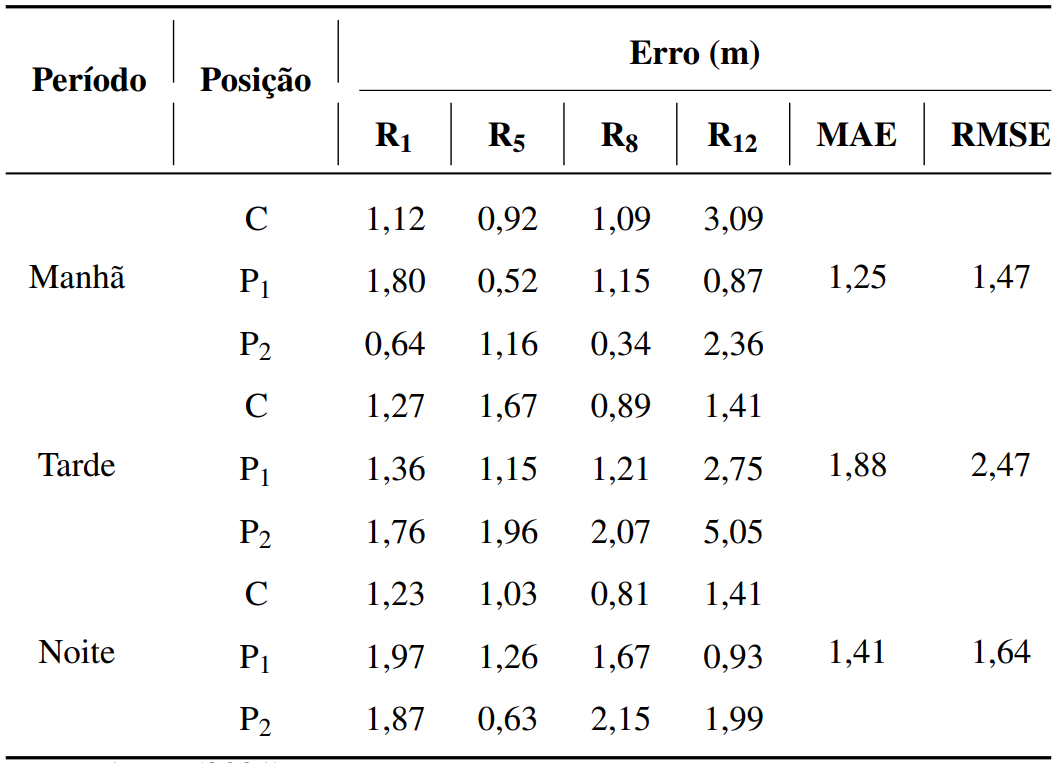
\includegraphics[width=8cm, height=3.9cm]{imgs/erros-localizacao.PNG}
			\vspace{-5pt}
			\caption*{\tiny{Fonte: Autor (2021).}}
			\vspace{-15pt}
		\end{figure}
		\begin{block}{}%{Aplicação da Técnica de Trilateração}
			\begin{itemize}[label=\textcolor{black}{\textbullet}, left=5pt]
				\justifying
				\item O menor erro de localização ocorreu no período da manhã (0,34 m) na posição R$_\text{8}$P$_\text{2}$;
				\item O maior erro de localização ocorreu no período da tarde (5,05 m) na posição R$_\text{12}$P$_\text{2}$;
				\item Percebe-se que houve variações nos erros de localização nos distintos períodos das capturas dos dados.%, podendo ser influenciado por fatores relativos a multi-percurso, temperatura e umidade do ambiente.
			\end{itemize}
		\end{block}
		
	\end{frame}

	\begin{frame}
		\frametitle{Resultados e Discussões}
		\framesubtitle{Aplicação da Técnica de Trilateração}
		\begin{figure}
			\caption*{Tabela 5: Comparação entre resultados obtidos com utilização e sem utilização dos métodos propostos para ajuste de erro de localização}
			\vspace{-5pt}
			\centering
			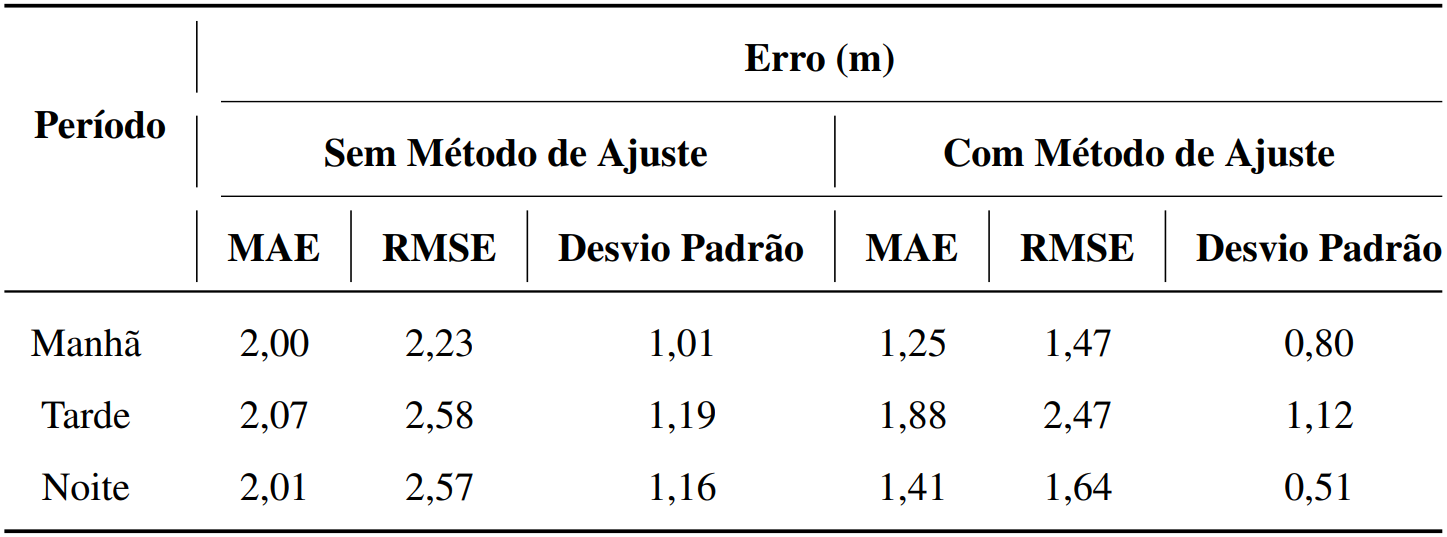
\includegraphics[width=8.5cm, height=3.6cm]{imgs/comparacao-metodos.PNG}
			\vspace{-5pt}
			\caption*{\tiny{Fonte: Autor (2021).}}
			\vspace{-15pt}
		\end{figure}
		
		\begin{block}{}%{Aplicação da Técnica de Trilateração}
			\begin{itemize}[label=\textcolor{black}{\textbullet}, left=5pt]
				\justifying
				%\item O menor erro de localização está no período da manhã (0,34 m) na posição R$_\text{8}$P$_\text{2}$;
				%\item O maior erro de localização está no período da tarde (5,05 m) na posição R$_\text{12}$P$_\text{2}$;
				%\item Percebe-se que houve variações nos erros de localização nos distintos períodos das capturas dos dados, podendo ser influenciado por fatores relativos a multi-percurso, temperatura e umidade do ambiente.
				%\item Realizou-se uma comparação dos métodos propostos de ajustes. Observa-se uma redução do erro de localização em cada período: manhã (34,08\%), tarde (4,26\%) e noite (36,19\%);
				\item Observa-se uma redução do erro de localização em cada período: manhã (34,08\%), tarde (4,26\%) e noite (36,19\%);
				\item No geral houve uma redução de 24,83\% no erro médio
				de localização.%, indicando viabilidade de tais métodos.
			\end{itemize}
		\end{block}
		
	\end{frame}

	\begin{comment}
	\begin{frame}
		\frametitle{Resultados e Discussões}
		\framesubtitle{Aplicação da Técnica de Trilateração}
		\begin{block}{}%{Aplicação da Técnica de Trilateração}
			\begin{itemize}[label=\textcolor{black}{\textbullet}]
				\justifying
				\item Período da tarde houve um maior erro de localização e de desvio padrão;
				\item Assim, pode-se inferir que o período de mapeamento (fase \textit{offline}) não influencia diretamente na redução do erro de localização obtido na fase \textit{online};
				\item Visto que esse procedimento foi realizado no período da tarde, onde obteve-se o maior erro de localização.
			\end{itemize}
		\end{block}
	\end{frame}
	\end{comment}
	
	\begin{frame}
		\frametitle{Resultados e Discussões}
		\framesubtitle{Aplicação da Técnica de Trilateração}
		\begin{figure}
			\caption*{Figura 10: Erro de localização e desvio padrão por período}
			\vspace{-5pt}
			\centering
			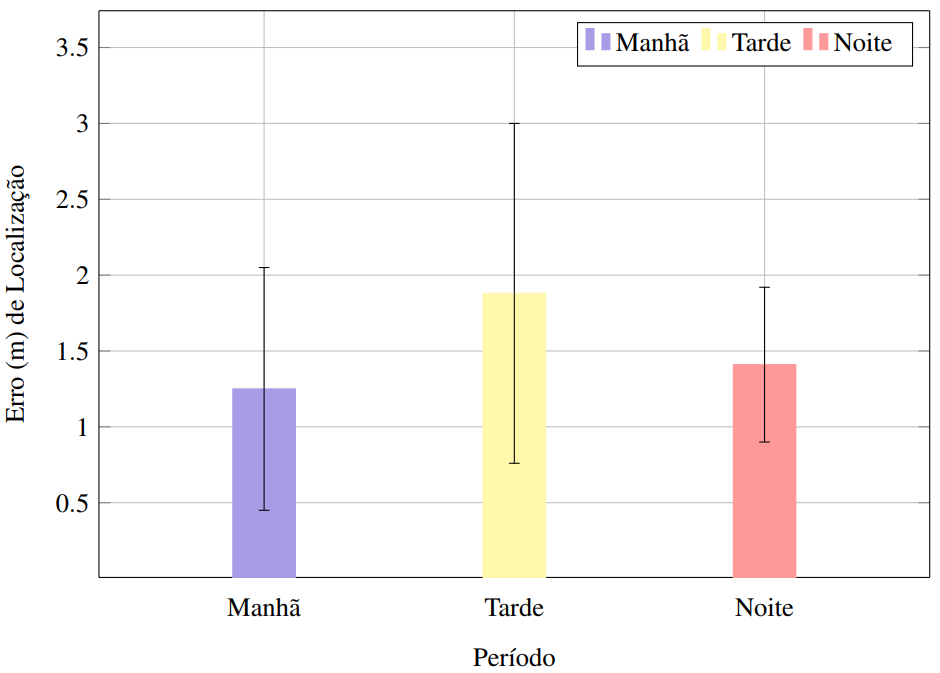
\includegraphics[width=8.5cm, height=6.4cm]{imgs/grafico_final.PNG}
			\vspace{-5pt}
			\caption*{\tiny{Fonte: Autor (2021).}}
		\end{figure}
	\end{frame}
	
	\section{Considerações Finais}
	\label{consideracoes-finais}
	\begin{frame}
		\frametitle{Considerações Finais}
		%\begin{block}{}
			\begin{itemize}[label=\textcolor{black}{\textbullet}, left=0pt]
				\justifying
				\item {\footnotesize No \textit{fingerprint} a região com maior acurácia foi a região 1 (91,67\%) e a região de menor acurácia foi a região 5 (42,22\%);}
				%\item A região \textit{fingerprint} a região com maior acurácia foi a região 1 (91,67\%) e a região de menor acurácia foi a região 5 (42,22\%);
				\item {\footnotesize Assim, percebe-se que o período de coleta dos RSSIs não influencia diretamente na classificação das regiões, bem como na redução do erro de localização;}
				\item {\footnotesize Isso pode ocorrer devido à complexidade do ambiente interno, relativo a fatores que impactam no sinal propagado;}
				\item {\footnotesize O erro de localização utilizando a métrica RMSE: 1,47 m pela manhã, 2,47 m pela tarde e 1,64 m pela noite;}
				\item {\footnotesize Ressalta-se que os métodos propostos contribuíram significativamente com a minimização do erro médio de localização obtido, alcançando uma redução geral de 24,83\%;}
				%\item {\footnotesize Este trabalho apresentou resultados satisfatórios, sendo que a precisão obtida mostrou-se semelhante a outros trabalhos, que utilizaram as mesmas tecnologias e técnicas.}
			\end{itemize}
		%\end{block}
	\end{frame}
	\begin{frame}
		\frametitle{Considerações Finais}
		\begin{block}{Trabalhos Futuros}
			\begin{itemize}[label=\textcolor{black}{\textbullet}, left=5pt]
				\justifying
				\item Analisar outros modelos de propagação de sinal que possam oferecer uma melhor caracterização do ambiente \textit{indoor};
				\item Aplicar filtros para reduzir os ruídos dos dados coletados; 
				\item Analisar possíveis métodos para minimizar a onerosidade
				no processo de mapeamento do \textit{fingerprint};
				\item Implementar um sistema de localização em tempo
				real para um ambiente \textit{indoor}, utilizando as técnicas em conjunto.
			\end{itemize}
		\end{block}
	\end{frame}

	\section{Referências}
	\label{referencias}
	\begin{frame}
		\frametitle{Referências}
		\begin{itemize}[left=0pt]%[label=\textcolor{black}{\textbullet}, left=5pt]
			\setlength\itemsep{5pt}
			\justifying
			
			\item {\footnotesize ARAVENA, C. A.; DELAZARI, L. S. Desenvolvimento de aplicativo para auxílio à navegação em ambientes internos. \textbf{Revista Brasileira de Cartografia}, [\textit{s. l.}], v. 73, n. 2, p. 530-541, 2021.}
			
			\item {\footnotesize BARROS, A. C. G. D. A. \textbf{Proposta de Técnica de Localização Interna para dispositivos móveis utilizando redes locais sem fio}. 2016. Dissertação de Mestrado (Mestrado em Ciêcia da Computação) – Universidade Federal de Pernambuco, Recife, PE, 2016.}
			
			\item {\footnotesize BERZ, E. L. \textbf{Sistema Híbrido de localização indoor baseado em RFID e análise visual}. 2015. Tese (Doutorado em Ciência da Computação) – Pontifícia Universidade Católica do Rio Grande do Sul, Porto Alegre, RS, 2015}
			
			\item {\footnotesize MARI, S. K.; KIONG, L. C.; KIM, L. H. A hybrid trilateration and fingerprinting approach for indoor localization base on wifi. \textbf{Fourth International Conference on Advances in Computing, Comunication Automation - ICACCA}, Subang Jaya, p. 1-6, 2018.}
			
		\end{itemize}
	\end{frame}

	\begin{frame}
		\frametitle{Referências}
		\begin{itemize}[left=0pt]%[label=\textcolor{black}{\textbullet}, left=5pt]
			\setlength\itemsep{5pt}
			\justifying
			
			\item {\footnotesize MITTELSTADT, R. S. \textbf{BLUEPATH}: Sistema de localização indoor. 2018. Monografia (Curso de Engenharia de Computação) – Universidade do Vale do Taquari - UNIVATES, Lajeado, RS, 2018.}
			
			\item {\footnotesize MOREIRA, F. M.; FARIAS, M. S.; CARVALHO, P. V. R. Posicionamento em Ambientes Internos com Dispositivos Wi-Fi de Baixo Custo. \textbf{International Nuclear Atlantic Conference - INAC}, Belo Horizonte, MG, n. 13, p. 22-27, 2017.}
			
			\item {\footnotesize SADOWSKI, S.; SPACHOS, P. RSSI-Based Indoor Localization With the Internet of Things. \textbf{IEEE Access}, Canada, v. 6, p. 30149-30161, 2018.}
			
			\item {\footnotesize WEERASINGHE, Y. S. P.; DISSANAYAKE, M. B. Towards IoT; Comparison of RSS based indoor localization using supervised learning and trilateration in WSN. \textbf{International Conference on Industrial an Information Systems - ICIISS}, Perandeniy, Sri Lanka, p. 290-295, 2019.}
			
		\end{itemize}
	\end{frame}

	\section{Agradecimentos}
	\label{agradecimentos}
	\begin{frame}
		%\frametitle{Obrigado pela Atenção!}
		\frametitle{Agradecimentos}
		\begin{block}{Duvidas, sugestões, questionamentos?}
			\centering
			{\Large Obrigado pela Atenção!}
		\end{block}
		%Duvidas, sugestões, questionamentos?
		\vspace{-20pt}
		\begin{figure}
			\centering
			
\includegraphics[width=0.55\linewidth]{imgs/homer.png}
		\end{figure}
	\end{frame}
		
	
\begin{comment}
	\subsection{Microcontrolador MCF51CN P2}
	\begin{frame}
		\frametitle{Microcontrolador MCF51CN}
		%imgs uma ao lado da outra
		\begin{figure}
			\centering
			\hspace{0.7cm}\parbox{5cm}{\centering\includegraphics[width=0.8\linewidth]{imgs/chip.jpg}
			\caption{Chip MCF51CN}}
			\qquad
			\begin{minipage}{5cm}
				\flushleft
				\includegraphics[width=4cm, height=2.8cm]{imgs/chip_full.jpg}
				\caption{Dispositivo MCF51CN128 \textit{ColdFire}}
			\end{minipage}
		\end{figure}
	\end{frame}
	
	\section{Características}
	
	\subsection{Memórias}
	\begin{frame}
		\frametitle{Características}
		\framesubtitle{Memórias}
		
		\begin{itemize}[label=\textcolor{black}{\textbullet}]
			\item Memória \textit{Flash}: 128 KB;
			\item Memória RAM: 24 KB;
			\item \textit{Flash} utiliza tensão e temperatura de operação total para Leitura/Programação/Apagamento;
			\item Circuito de segurança contra acessos não autorizados a RAM e conteúdos da \textit{Flash}.
		\end{itemize}
	\end{frame}

	\subsection{Frequências}
	\begin{frame}
		\frametitle{Características}
		\framesubtitle{Frequências}
		
		\begin{itemize}[label=\textcolor{black}{\textbullet}]
			\item 32-bit - \textit{ColdFire} \normalfont{$V_{1}$} CPU;
			\item Frequências de \textit{clocks}:
			\begin{itemize}%[label=\textcolor{black}{\textbullet}]
				\item[$\circ$] 50,33 MHz $\Rightarrow$ Para tensões entre 3.6V a 3.0V;
				\item[$\circ$] 40 MHz $\Rightarrow$ Para tensões entre 3.0V a 2.1V;
				\item[$\circ$] 20 MHz $\Rightarrow$ Para tensões entre 2.1V a 1.8V;
				\item[$\circ$] Executa 2,1 MIPS por MHz
				\item[$\circ$] Faixa de temperatura de atuação -40ºC a 85ºC.
			\end{itemize}
			\item Oscilador (XOSC): cristal ou ressonador cerâmico atuando entre 31,25 KHz a 38,4 KHz ou 1 MHz a 25 MHz;
		\end{itemize}
	\end{frame}
	
	\subsection{Periféricos (IO)}
	\begin{frame}
		\frametitle{Características}
		\framesubtitle{Periféricos (IO)}
		\begin{itemize}[label=\textcolor{black}{\textbullet}]
			\item Possui até 70 pinos I/O de uso geral (GPIO) com controle de pin mux; 
			\item Possui 16 pinos de interrupção de teclado (KBI);
			\item Possui 16 pinos Rapid (GPIO) de alta velocidade atuando em \textit{toggle};
			%\item Interface Ethernet - Operando em half ou full duplex;
			%\item External Bus - Interface de barramento externo.
			\item Possui 3 módulos de pausa operacinal SCI 13bits;
			\item Possui 2 interfaces \textit{full-duplex} ou bi-direcional SPI, atuando com mester ou escravo;
			\item Possui 2 módulos de 3 canais(16bits) para captura de entrada e comparação de saída PWM;
			\item Possui 1 módulo sincronização de relógio externo RTC-8bits;
			\item Possui 2 temporizadores modulares(8bits) MTIM.
		\end{itemize}
	\end{frame}

	\subsection{Gerenciamento de Energia}
	\begin{frame}
		\frametitle{Características}
		\framesubtitle{Gerenciamento de Energia}
		\begin{itemize}[label=\textcolor{black}{\textbullet}]
			\item Possui dois modos de paragem de baixa potência; 
			\item Modo de espera de energia reduzida para execução de todos os periféricos;
			\item Modo de baixo consumo, permitindo que os periféricos funcionem enquanto o regulador de tensão esteja em standby;
			\item Oscilador externo de baixa potência, pode ser usado em modo parada para ativação dos periféricos; 
			\item Pinos e \textit{clocks} para periféricos não disponíveis são desativados automaticamente para reduzir o consumo; 
		\end{itemize}
	\end{frame}

	\section{Aplicações}
	\subsection{FreeMASTER}
	\begin{frame}
		\frametitle{Aplicações}
		\begin{block}{FreeMASTER - Implementação driver serial}
			\begin{itemize}[label=\textcolor{black}{\textbullet}]
				\item Ferramenta de desenvolvimento baseada em comunicação com PC, que utilizada ferramentas gráficas e monitoramento para aplicações embarcadas;		
				\item Pode-se utilizar outras bibliotecas e APIs;
			\end{itemize}
		\end{block}
		\begin{figure}
			\centering
			\includegraphics[width=1\linewidth]{imgs/app1.png}
			\caption{Descrição para adicionar driver serial na aplicação do sistema embarcado}
		\end{figure}
	\end{frame}

	\subsection{Serial para Ethernet}
	\begin{frame}
		\frametitle{Aplicações}
		\begin{block}{Serial para Ethernet em modo bridge}
			\begin{itemize}[label=\textcolor{black}{\textbullet}]
				\item Utiliza RTOS FreeRTOS{\small \texttrademark}(\textit{Open Source}) e TCP/IP, com portas seriais UART e SPI. A conexão ocorre através da implementação de \textit{sockets}. 
				\item O FreeRTOS é um kernel do sistema operacional em tempo real para sistemas embarcados. Disponível para várias plataformas de microcontroladores.
			\end{itemize}
		\end{block}
		\begin{figure}
			\centering
			\includegraphics[width=0.8\linewidth]{imgs/app2.png}
			\caption{Placa para uso em modo \textit{bridge}}
		\end{figure}
	\end{frame}
	
	\section{Ferramentas}
	\subsection{UMultilink}
	\begin{frame}
		\frametitle{Ferramentas}
		\begin{block}{Interface de Desenvolvimento Universal - UMultilink}
			\begin{itemize}[label=\textcolor{black}{\textbullet}]
				\item O USB Multilink é uma interface de depuração e programação fácil que permite a comunicação através de conexão USB;
				\item Ótimo para desenvolvimento por conta da velocidade e confiabilidade;
			\end{itemize}
		\end{block}
		\begin{figure}
			\centering
			\includegraphics[width=0.7\linewidth]{imgs/Multilink.png}
			\caption{Dispositivo multilink}
		\end{figure}
	\end{frame}

	\subsection{Eclipse IDE}
	\begin{frame}
		\frametitle{Ferramentas}
		\begin{itemize}[label=\textcolor{black}{\textbullet}]
			\item CodeWarrior para MCUs (Eclipse IDE): 
			\begin{itemize}
				\item[$\circ$] IDE integra as ferramentas de desenvolvimento para diversas arquitetura;
				\item[$\circ$] Eclipse IDE 4.2.1 (Juno);
				\item[$\circ$] Código Assembler;
				\item[$\circ$] Copilador e depurador C/C++;
				\item[$\circ$] Programação \textit{flash} integrada;
			\end{itemize}
			\item CodeWarrior para MCUs (Clássica IDE); 
			\item Software de programação em circuito  \textit{flash};
		\end{itemize}
	\end{frame}
	
	\begin{frame}
		\frametitle{Ferramentas}
		\begin{figure}
			\centering
			\parbox{5cm}{\vspace{0.2cm}\includegraphics[width=5cm, height=3.55cm]{imgs/ide.jpg}\vspace{-0.2cm}
			\caption{IDE Eclipse}}
			\qquad
			\begin{minipage}{5cm}
				\flushright
				\includegraphics[width=1\linewidth]{imgs/ide_c.png}
				\caption{IDE Clássica}
			\end{minipage}
		\end{figure}
	\end{frame}
	
	\subsection{Freescale Tower System}
	\begin{frame}
		\frametitle{Ferramentas}
		\begin{block}{Sistema Freescale Tower}
			\begin{itemize}[label=\textcolor{black}{\textbullet}]
				\item Sistema modular para plataforma de desenvolvimento de microcontroladores 8,16 e 32 bits;
				\item Permite o desenvolvimento e prototipagem rápida;
				\item Módulos são fáceis de se usar e reconfiguráveis; 
				\item Hardware \textit{Open Source}.
			\end{itemize}
		\end{block}
		\begin{figure}
			\centering
			\includegraphics[width=6.5cm, height=3.5cm]{imgs/tower.jpg}
			\caption{\textit{Freescale Tower System}}
		\end{figure}
	\end{frame}

	\section{Referências}
	\begin{frame}
		\frametitle{Referências}
		\begin{itemize}[label=\textcolor{black}{\textbullet}]
			\item MCF51CN128: 32-bit ColdFir. V1 Microcontrollers. Disponível em: \url{http://bit.ly/3bOs43G}. Acesso em: 17 Fevereiro de 2020.
			\item Data Sheet: MCF51CN128 ColdFire
Microcontroller
Cover: MCF51CN128. Disponível em: \url{http://bit.ly/2P73YY1}. Acesso em: 17 Fevereiro de 2020.
			\item Tools and Software: MCF51CN128. Disponível em: \url{http://bit.ly/39LJPyu}. Acesso em: 18 Fevereiro de 2020.
		\end{itemize}	
	\end{frame}
	
\end{comment}

\end{document}